\documentclass[oneside, 12pt]{book}

% ------------------------------------------------------------------------------
% Setup for table of contents
\setcounter{tocdepth}{3} 	% TOC should label down to subsubsections
\setcounter{secnumdepth}{2}	% TOC should not number further than a subsection number
% ------------------------------------------------------------------------------

\usepackage[english]{babel}
\usepackage{amsfonts, amsmath, amsthm}	% For properly formatting symbols, theorems, lemmas, and definitions
\usepackage{enumitem} 					% For listing items and sub-items
\usepackage{hyperref} 					% For inserting links
\usepackage{fullpage}					% For setting up reasonable margins
\usepackage{graphicx} 					% For inserting images
\usepackage{float}						% For forcing image location

% Some useful commands
\newcommand{\abs}[1]{\left|#1\right|}	% Absolute value
\newcommand{\norm}[1]{\abs{\abs{#1}}} 	% Use double-bar notation for vector magnitude
\newcommand{\R}{\mathbb{R}}

% Theorems, Definitions, and Lemmas should not be numbered
\newtheorem*{theorem}{Theorem}
\newtheorem*{definition}{Definition}
\newtheorem*{lemma}{Lemma}

\begin{document}
% Title page setup
\title{Multivariable Calculus: A Summary}
\author{William Boyles}
\date{}

\frontmatter
\maketitle

\tableofcontents

\mainmatter
	\chapter{Background \& Review}
Everything mentioned in this chapter should already be familiar to you from other math classes.
These topics span two major areas: algebra/pre-calculus and limits.
Ideas from these topics will often be used implicitly or without a passing reference. \\

If you are unfamiliar with anything mentioned, you can use many of the great online resources like Khan Academy to familiarize yourself before moving forward.

\section{Algebra and Pre-Calculus}
\noindent

\subsection{Sets}
\begin{definition}
	A set $A$ is a collection of distinct elements. Those elements can be anything, like numbers, functions, and even other sets.
\end{definition}
We can define a set by giving its elements, like $A = \{-2, 5, 3\}$ or by describing its properties, like $A = \{x \mid x > 0\}$ where the vertical bar means "such that".
If an object $x$ is a member of the set $A$, we write $x\in A$.\bigskip


\noindent
A set $A$ is called a subset of a set $B$ if every element of $A$ is also an element of $B$. 
We can write this as $A \subseteq B$. 
For example, $\{7, 10, 16\} \subseteq \{5, 6, 7, 9, 10, 11, 16\}$. 
Note that this relation can be strict if there exists at least one element in $B$ that is not also an element of $A$. 
Some common sets and their informal definitions are given below:

\begin{table}[H]
	\centering
	\begin{tabular}{c|c|c}
		Set Name & Symbol & Informal Definition                                                                                                                         \\ \hline
		Natural numbers & $\mathbb{N}$ & $\{1, 2, 3, \dots\}$           						                                                                        \\
		Integers & $\mathbb{Z}$ & $\{\dots, -3, -2, -1, 0, 1, 2, 3, \dots\}$                                                                                            \\
		Rational numbers & $\mathbb{Q}$ & $\{\frac{m}{n} \mid m,n \in\mathbb{Z}$ and $n \neq 0\}$                                                                       \\
		Real numbers & $\mathbb{R}$ & Any number on the number line\footnote{Sadly, there is no way to give a stronger formal definition without higher mathematics.}   \\
	\end{tabular}
\end{table}

This means that $\mathbb{N} \subset \mathbb{Z} \subset \mathbb{Q} \subset \mathbb{R}$.\bigskip


\noindent
There are several common operations that can be performed on sets.
The union $A \cup B$ of two sets $A$ and $B$ is the set of all elements that are elements of $A$ or of $B$. 
Similarly, the intersection $A \cap B$ of two sets $A$ and $B$ is the set of all elements that are also elements of both $A$ and $B$.
\begin{example}
	If $A = \{\sqrt{2}, 2, 5, 8\}$ and $B = \{-9, 8, 2.3\}$, what are $A \cup B$ and $A \cap B$?		
\end{example}
To find the union, we combine the sets, making sure to include any repeated element only once:
\begin{equation*}
	A \cup B = \{-9, \sqrt{2}, 2, 2.3, 5, 8\}.
\end{equation*}
Then, since the only element both sets share is 8, we also have
\begin{equation*}
	A \cap B = \{8\}.
\end{equation*}

\subsection{Intervals}
\begin{definition}
	We call a subset $I$ of $\mathbb{R}$ an interval if, for any $a, b \in I$ and $x \in \mathbb{R}$ such that $a \leq x \leq b$, then $x \in I$. 
\end{definition}
We can write an interval more simply using the notation $[a, b]$, which is equivalent to $\{x \in \mathbb{R} \mid a \leq x \leq b\}$. 
This is called a closed interval, and to make the inequalities strict, we can also define an open interval by using parantheses instead of square brackets.\bigskip

In addition, we can mix the two to create half-open intervals, where one inequality is strict and the other isn't. 
For instance, $(2, 5]$ refers to the set $\{x \in \mathbb{R} \mid x < 2 \leq 5\}$
Finally, if the interval is unbounded in either direction, we use the notations $-\infty$ and $\infty$ to indicate that there is no minimum or maximum, respectively.

\begin{example}
	Is $8 \in (-\infty, 4) \cup [8, 100)$?
\end{example}
\begin{answer}
	Since $8 \leq 8 < 100$ is a true statement, $8 \in [8, 100)$. 
	Since we are taking the union with another set, all of the members of the right interval will also be members of the union of intervals. 
	Therefore, the statement is true.
\end{answer}                       % Sets
\subsection{Functions}
\begin{definition}
    A function $f$ is a rule between a pair of sets, denoted $f: D \to C$, that assigns values from the first set, the domain $D$, to the second set, the codomain $C$.
\end{definition}

We call the subset of the codomain $C$ that constitutes all values $f$ can actually attain the range $R \subseteq C$. 
Note that when we draw a graph of a function, all we are doing is drawing all ordered pairs $\{(x, f(x)) \mid x \in D\}$.

\begin{example}
    Find the domain of the following function:
    \begin{equation*}
        f(x) = \frac{1}{(1 - x)\sqrt{5 - x^2}}
    \end{equation*}
\end{example}

\begin{answer}
    We know that $\frac{n}{0}$ is undefined for all $n \in \mathbb{R}$ and $\sqrt{x}$ is only defined for $x \geq 0$. 
    The first condition applies to the first term in the denominator and both conditions apply to the second, giving us
    \begin{equation*}
        (1 - x) \neq 0 \text{ and } 5 - x^2 > 0
    \end{equation*}
    The first condition implies $x \neq 1$ while the second implies $|x| < \sqrt{5}$.
    Putting these together, we find that the domain is
    \begin{equation*}
        \{x \mid x \neq 1, |x| < \sqrt{5}\} \text{ or } (-\sqrt{5}, 1) \cup (1, \sqrt{5})
    \end{equation*}
\end{answer}

We can also compose two functions, such that the ouput of one function is the input of another: 
\begin{equation*}
    (f \circ g)(x) = f(g(x)).
\end{equation*}

\begin{definition}
    A function $g$ is called an inverse function of $f$ if $f(g(x)) = x$ for all x in the domain of g and $g(f(x))$ for all x in the domain of f. 
    We write this as $g = f^{-1}$.
\end{definition}

One common algorithm for finding an inverse function is to set $y = f(x)$, substitute all $x$'s for $y$'s, and then solve for y.
\begin{example}
    Find the inverse function of 
    \begin{equation*}
        f(x) = \frac{5x + 2}{4x - 3}.
    \end{equation*}
\end{example}
\begin{answer}
    We first make the substitutions to set up the algorithm:
    \begin{equation*}
        y = \frac{5x + 2}{4x - 3} \text{ followed by }
        x = \frac{5y + 2}{4y - 3}
    \end{equation*}
    After multiplying both sides by the denominator and simplifying, we have
    \begin{equation*}
        \implies 4xy - 3x = -5y - 2 \\
        \implies y = f^{-1}(x) = \frac{3x - 2}{4x + 5}.
    \end{equation*}
\end{answer}

We say that a function $f$ is even if it satisfies $f(-x) = f(x)$ for all $x \in D$.
Likewise, we say that a function $f$ is odd if it satisfies $f(-x) = -f(x)$ for all $x \in D$. 
Geometrically, we can see that the graph of an even function is symmetric with respect to the $y$-axis, while the graph of an odd function is symmetric with respect to the origin. 

\begin{example}
    Is $f(x) = 2x - x^2$ even, odd, or neither?
\end{example}
\begin{answer}
    \begin{equation*}
        f(-x) = 2(-x) - (-x)^2 = -2x - x^2
    \end{equation*}
    Since $f(-x) \neq f(x)$ and $f(-x) \neq -f(x)$, the function is neither even nor odd.
\end{answer}                   % Functions
\subsection{Complex Numbers}
\begin{definition}
	$i$ is called the imaginary unit. It's defined by $i^2 = -1$.
\end{definition}


\noindent
Complex numbers ($\mathbb{C}$) have the form $z = \alpha + \beta i$, where $\alpha$ and $\beta$ are real numbers. The $\alpha$ part of $z$ is called the real part, so $\Re(z) = \alpha$. The $\beta$ part of $z$ is called the imaginary part, so $\Im(z) = \beta i$.\\

\noindent
Often, complex numbers are visualized as points or vectors in a 2D plane, called the complex plane, where $\alpha$ is the x-component, and $\beta$ is the y-component. Thinking of complex numbers like points helps us define the magnitude of complex numbers and compare them. Since a point $(x,y)$ has a distance $\sqrt{x^2+y^2}$ from the origin, we can say the magnitude of $z$, $\lvert z \rvert$ is $\sqrt{\alpha^2 + \beta^2}$. Thinking of complex numbers like vectors helps us understand adding two complex numbers, since you just add the components like vectors.\\

\noindent
A common operation on complex numbers is the complex conjugate. The complex conjugate of $z = \alpha + \beta i$ is $\overline{z} = \alpha - \beta i$. $z$ and $\overline{z}$ are called a conjugate pair.\\

\noindent
Conjugate pairs have the following properties.
Let $z, w \in \mathbb{C}$.
\begin{align*}
	\overline{z \pm w} &= \overline{z} \pm \overline{w} \\
	\overline{zw} &= \overline{z}\overline{w} \\
	\overline{z} &= z \Leftrightarrow z \in \mathbb{R} \\
	z\overline{z} &= \lvert z \rvert^2 = \lvert \overline{z} \rvert^2 \\
	\overline{\overline{z}} &= z \\
	\overline{z}^n &= \overline{z^n} \\
	z^{-1} &= \frac{\overline{z}}{\lvert z \rvert^2} 
\end{align*}
 			% Complex Numbers
\subsection{Factoring Polynomials}
\noindent
We want to break up a polynomial like $f(x) = a_0 + a_1x^1 + \ldots a_nx^n$ into linear factors so that $f(x) = c(x-b_1)\cdot \ldots \cdot(x - b_n)$. This form makes it simple to see that the roots of $f$, solutions to $f(x) = 0$, are $x = b_1 \ldots b_n$.\\

\noindent
For quadratics, $f(x) = ax^2 + bx + c$, there exists a simple formula that will give us both roots, the quadratic formula
\begin{equation*}
	x = \frac{-b \pm \sqrt{b^2-4ac}}{2a}.
\end{equation*}

\noindent
We can see that when $b^2 - 4ac < 0$, like for $f(x) = x^2 + 5x + 10$, we will get complex roots $\alpha \pm \beta i$. For any polynomial, these roots come in pairs, so if $\alpha + \beta i$ is a root, then so is $\alpha - \beta i$. This means that every conjugate pair $\alpha \pm \beta i$ has a quadratic equation with those roots. Sometimes we will not factor quadratics with complex roots into linear terms.\\

\noindent
Although there do exist explicit formulas for finding roots for cubic (degree 3) and quartic (degree 4) equations, they are too long and not useful enough to memorize. When working by hand, we instead use other tricks to find roots.\\

\noindent
There are a few useful tricks that can help. If the polynomial doesn't have a constant term, then 0 is a root. If all the coefficients sum to 0, then 1 is a root. For certain polynomials with an even number of terms, like all cubics of the form $ax^3 + bx^2 + cax + cb$ we can factor out a term from the first two and last two terms to get $x^2(ax+b)+c(ax+b) = (ax+b)(x^2+c)$. For other polynomials, we might just try guessing and checking values. However, we need a more efficient way that works in general.\\

\noindent
Since we are looking to find linear factors $f(x) = (x-b_1)\cdot \ldots \cdot(x-b_n)$, we can see that the constant term in the polynomial is the product of the roots $b_1 \ldots b_n$. In fact, since the coefficients of polynomials are completely determined by the roots and the leading coefficient, all the coefficients are sums and products of roots. You might remember when factoring quadratics that the coefficient of $x$ term is the sum of the two roots. These rules are called Vieta's formulas.\\

\noindent
So, if we have the constant term, we can check all of its integer factors to see if any are roots. For each root, we can divide, using a technique like synthetic division, to continue finding the rest of the roots. This method is especially useful on tests because the roots tend to be integers.

\input{../common/algebraPreCalc/factoringPolynomials_example.tex} 		% Factoring Polynomials
\subsection{Trig Functions \& The Unit Circle}
\noindent
Imagine aa circle of radius 1 centered at the origin that we'll call the unit circle. The x and y coordinates of a point on the unit circle are completely determined by the angle $\theta$ in radians between the $x$-axis and a line from the origin to the point.\\

\noindent
The function $\cos{\theta}$ tells us x-coordinate of the point, while $\sin{\theta}$ tells us the y-coordinate of the point. The function $\tan{\theta} = \frac{\sin{\theta}}{\cos{\theta}}$ tells us the slope of the line from the origin to the point. Most of the trig functions have geometric interpretations as shown below. The most used ones are $\sin$, $\cos$, $\tan=\frac{\sin}{\cos}$, $\cot = \frac{\cos}{\sin}$, $\csc=\frac{1}{\sin}$, and $\sec=\frac{1}{\cos}$.

\begin{figure}[H]
	\label{unitCircle}
	\centering
	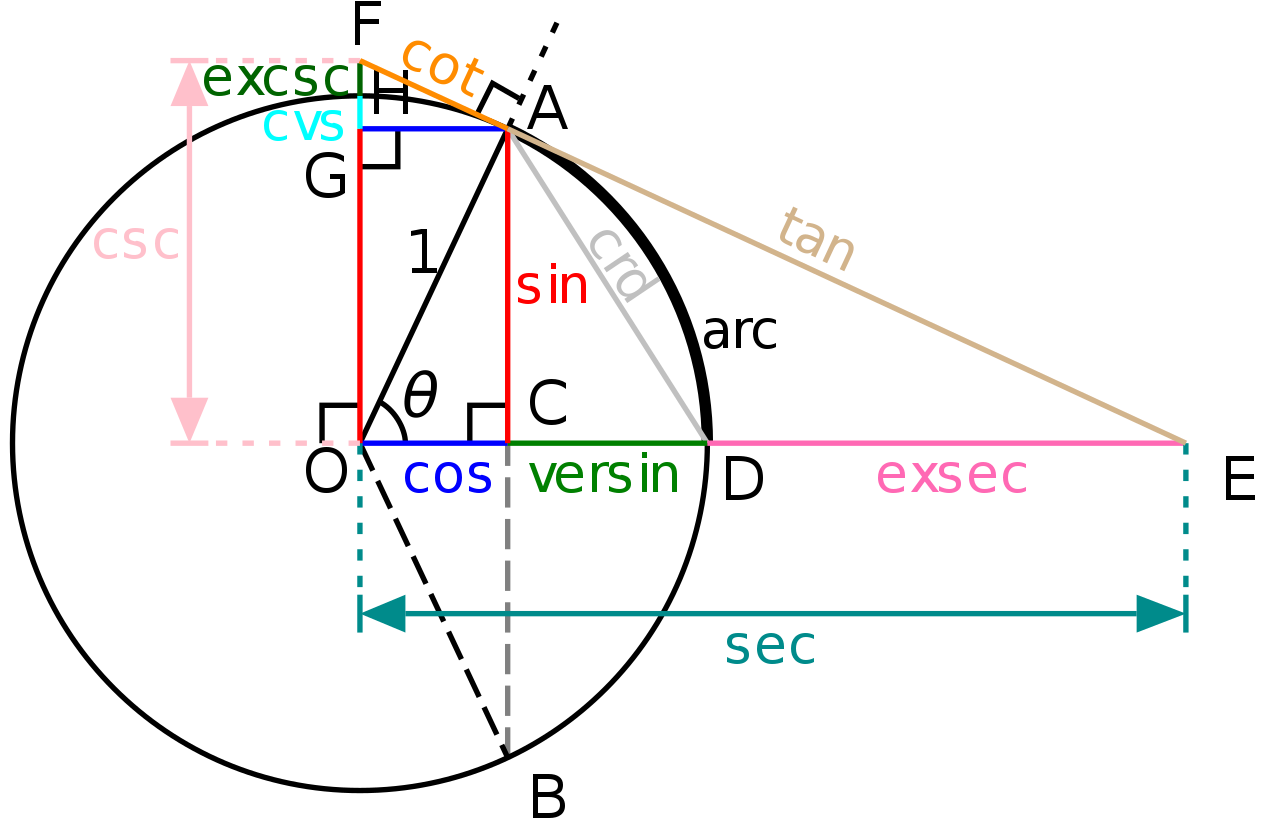
\includegraphics[width = 0.75\textwidth]{../common/algebraPreCalc/unitCircle2.png}
	\caption{\hyperref{https://en.wikipedia.org/wiki/Unit_circle}{}{}{Wikipedia - Unit circle}}
\end{figure}

\noindent
We can also think about the inverses of these trig functions. These are either notated with a -1 exponent on the function, or the prefix arc in front of the function name. Many of these functions are only defined on a part of the domain $\left[0, 2\pi\right]$. Below is a table of the inverse trig functions and their domains.

\begin{table}[H]
	\centering
	\begin{tabular}{l|l}
		Function  & Domain                                                 \\ \hline
		$\arcsin$ & $\left[-1, 1\right]$           						   \\
		$\arccos$ & $\left[-1, 1\right]$                                   \\
		$\arctan$ & $\left(-\infty, \infty\right)$                         \\
		$\arccot$ & $\left(-\infty, \infty\right)$                         \\
		$\arccsc$ & $\left(-\infty, -1\right] \cup \left[1, \infty\right)$ \\
		$\arcsec$ & $\left(-\infty, -1\right] \cup \left[1, \infty\right)$
	\end{tabular}
\end{table}
 	% Trig Functions / Unit Circle
\subsection{Trig Identities}
\noindent
As we could see in Figure \ref{unitCircle}, $\sin$ and $\cos$ form a right triangle with hypotenuse 1. So, using the Pythagorean Theorem,
\begin{equation*}
	\sin^2{\theta} + \cos^2{\theta} = 1.
\end{equation*}
By dividing by $\sin^2$ or $\cos^2$, we can also get
\begin{equation*}
	1 + \cot^2{\theta} = \csc^2{\theta} \text{ and } \tan^2{\theta} + 1 = \sec^2{\theta}.
\end{equation*}
Together, these 3 identities are called the Pythagorean Identities.\\

\noindent
We can also relate functions and co-functions.
\begin{equation*}
	\text{xxx}(\theta) = \text{coxxx}\left(\frac{\pi}{2} - \theta\right).
\end{equation*}

\noindent
Some of the most useful and used identities are the sum and difference.
\begin{align*}
	\sin{\left(\alpha \pm \beta\right)} &= \sin{\alpha}\cos{\beta} \pm \cos{\alpha}\sin{\beta} \\
	\cos{\left(\alpha \pm \beta\right)} &= \cos{\alpha}\cos{\beta} \mp \sin{\alpha}\sin{\beta} \\
	\tan{\left(\alpha \pm \beta\right)} &= \frac{\tan{\alpha} \pm \tan{\beta}}{1 \mp \tan{\alpha}\tan{\beta}} \\
	\sin{\alpha} \pm \sin{\beta} &= 2\sin{\left(\frac{\alpha \pm \beta}{2}\right)}\cos{\left(\frac{\alpha \mp \beta}{2}\right)} \\
	\cos{\alpha} + \cos{\beta} &= 2\cos{\left(\frac{\alpha + \beta}{2}\right)}\cos{\left(\frac{\alpha - \beta}{2}\right)} \\
	\cos{\alpha} - \cos{\beta} &= -2\sin{\left(\frac{\alpha + \beta}{2}\right)}\sin{\left(\frac{\alpha - \beta}{2}\right)} \\
\end{align*} 			    % Trig Identites
\subsection{Exponentials \& Logarithms}
\begin{definition}
	e is the base of the natural logarithm. It's defined by the limit
	\begin{equation*}
		e = \lim\limits_{n\rightarrow\infty}{\left(1+\frac{1}{n}\right)^n}.
	\end{equation*}
\end{definition}
\noindent
$\exp{x} = e^x$ and $\ln{x}$ are inverse functions of each other such that
\begin{equation*}
	e^{\ln{x}} = x \text{ and } \ln{e^x} = x.
\end{equation*}

\noindent
Just like other exponentials, the normal rules for adding, subtracting, and multiplying exponents apply:
\begin{equation*}
	e^xe^y = e^{x+y} \text{, } \frac{e^x}{e^y}=e^{x-y} \text{, and } \left(e^x\right)^k=e^{xk}.
\end{equation*}

\noindent
Similar rules apply for logarithms:
\begin{equation*}
	\ln{x}+\ln{y} = \ln{xy} \text{, } \ln{x}-\ln{y} = \ln{\left(\frac{x}{y}\right)} \text{, and } \ln{\left(a^b\right)} = b\ln{a}.
\end{equation*}

\noindent
We can also write a logarithm of any base using natural logarithms:
\begin{equation*}
	\log_{b}{a} = \frac{\ln{a}}{\ln{b}}.
\end{equation*}

\noindent
$e$ is also unique in that it is the only real number $a$ satisfying the equation
\begin{equation*}
	\frac{\mathrm{d}}{\mathrm{d}x}a^x = a^x,
\end{equation*}
meaning $e^x$ is its own derivative. 		% Exponential and logarithms
\subsection{Partial Fractions}
\noindent
If we have a function of two polynomials $f(x) = \frac{P(x)}{Q(x)}$, it's often easier to break this quotient into a sum of parts where the denominator is a linear or quadratic factor and the numerator is always a smaller degree than the denominator.

\begin{example}
	\begin{equation*}
		\frac{2x-1}{x^3-6x^2+11x-6} = \frac{1/2}{x-1}+\frac{-3}{x-2}+\frac{5/2}{x-3}.
	\end{equation*}
\end{example}

\noindent
One natural way to find these small denominators comes from the linear factors of the denominator where we keep quadratics with complex roots.
This way, when making a common denominator, we get back the original big denominator.
However, there are a few special cases we have to take care of.

\input{../common/algebraPreCalc/linearFactors.tex}
\input{../common/algebraPreCalc/repeatedLinearFactors.tex}
\input{../common/algebraPreCalc/quadraticFactors.tex}
\input{../common/algebraPreCalc/repeatedQuadraticFactors.tex}
\input{../common/algebraPreCalc/improperFractions.tex}
 			% Partial Fractions % Algebra and Pre-Calc
	\chapter{Vector-Valued Functions (VVFs)}
\section{Lines \& Planes as VVFs}
\noindent
VVFs are parametric equations that take one input value and return one or more output values as a vector. We can draw curves in space by defining the tail of the output of the VVF be at the origin and have the tip trace out the curve. We will look at some simple VVFs that you need to be able to recognize.\\
\subsection{Lines}
\noindent
A straight line is probably the simplest 3D VVF. We can form any straight line using a point that the line passes through and the direction vector of the line.\\
Letting $P$ be the point and $\vec{v}$ be the direction, a straight line has the form $\vec{r}(t) = \vec{P}+t\vec{v}$, where $\vec{P}$ is the vector with components the same as $P$. The function's output starts at $\vec{P}$ when $t=0$ and moves in the direction of $\vec{v}$ as $t$ increases.

% It'd be nice if we could get this image to fit on the above page
\begin{figure}[h]
	\centering
	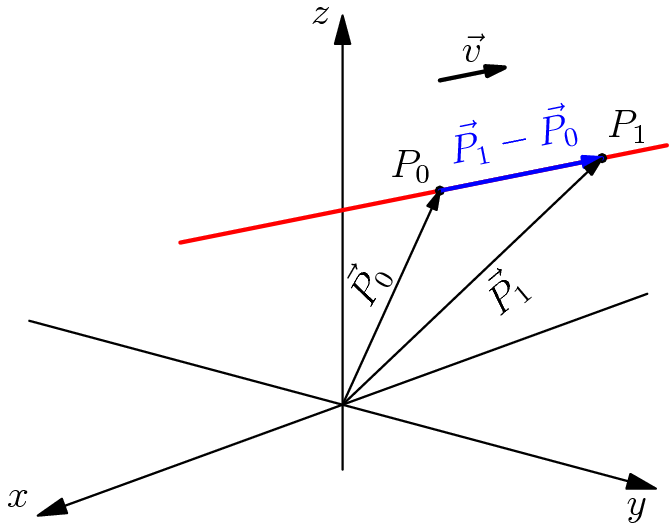
\includegraphics[scale=0.33]{Images/vectorValuedFunctions/VectorLine}
\end{figure}

\noindent
A line can also be formed using two points. To find the equation of the line in this case, let $\vec{v}$ be the vector connecting the two points, and let $\vec{P}$ be a vector point from the origin to one of the two points. We now have an origin point and direction and can write our function as
\begin{equation*}
	\vec{r}(t) = \vec{P_0} + t\left(\vec{P_1} - \vec{P_0}\right)	
\end{equation*}
 Where $P_0$ and $P_1$ are the two points on the line.
\subsection{Planes}
\noindent
A plane can also be formed using a point in the plane, $P$, and a vector perpendicular to the plane, $\vec{n}$. All vectors $\langle x,y,z \rangle$ that originate from $P$ and remain in the plane must be perpendicular to $\vec{n}$, so their dot product with $\vec{n}$ would be 0. So, the point-normal form of a plane is $\vec{n}\cdot\left(\langle x,y,z \rangle - \vec{P}\right) = 0$.\\
\small{Note: Conventionally, $\vec{n}$ is a unit vector, $\hat{n}$.}

\begin{figure}[h]
	\centering
	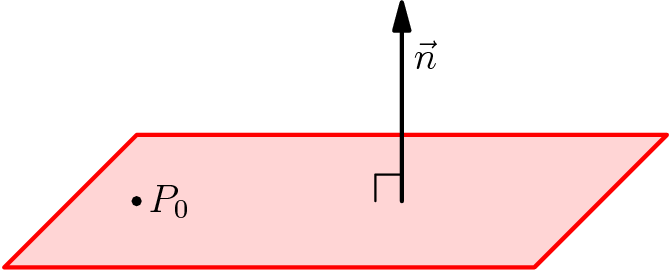
\includegraphics[scale=0.5]{Images/vectorValuedFunctions/PlaneNormalVector}
\end{figure}

\noindent
One can also construct a plane from 3 non-collinear points in the plane. One can still take advantage of point-normal form here by choosing 1 point to be $P_0$ and drawing vectors from this point to the two other points. The cross product of these two vectors is $\vec{n}$. $\left(\left(\vec{P_1} - \vec{P_0}\right) \times \left(\vec{P_2} - \vec{P_0}\right)\right) \cdot \left(\langle x,y,z \rangle - \vec{P_0}\right) = 0$ where $P_0$, $P_1$, and $P_2$ are the three points in the plane.\\

\noindent
One can also construct a plane from a point in the plane, $P_0$, and a line in the plane, $\vec{r}(t) = \vec{P_1} + t\vec{v}$, that doesn't pass through $P_0$. One can get this setup into point-normal form by choosing a an output of $\vec{r}(t)$, like $\vec{P_1}$, and constructing a vector that points from $\vec{P_1}$ to $\vec{P_0}$, $\vec{P_1}-\vec{P_0}$, and crossing this with $\vec{v}$ to find $\vec{n}$. $\left(\vec{v} \times \left(\vec{P_1} - \vec{P_0}\right)\right) \cdot \left(\langle x,y,z \rangle - \vec{P_0}\right) = 0$.\\

\noindent
One can also construct a plane from two intersecting lines, $\vec{r_1}(t) = \vec{P_0} + t\vec{v_1}$ and $\vec{r_2}(t) = \vec{P_0} + t\vec{v_2}$, where $P_0$ is where the two lines intersect. One can cross $\vec{v_1}$ with $\vec{v_2}$ to get the normal vector.
$\left(\vec{v_1} \times \vec{v_2}\right) \cdot \left(\langle x,y,z \rangle - \vec{P-0}\right) = 0$.
\section{Common Vector-Valued Functions}
\subsection{Circles}
\noindent
You should already recognize $x^2+y^2=r^2$ as the equation of a circle with radius $r$ centered at the origin. A circle as a VVF is $\vec{r}(t)=\langle r\cos{t}, r\sin{t} \rangle$, which is identical to the parametric form of a circle.\\
In $\mathbb{R}^3$, the z-component is some constant that tells us which plane, $z=c$, the circle is in.\\ 
We can also have circles parallel to $x=0$ and $y=0$ planes by changing the positions of the $\sin$, $\cos$, and $c$ terms. For example, $\vec{r}(t)=\langle \cos{t}, c, \sin{t}$ is a circle in the $y=c$ plane.
\subsection{Helices}
\noindent
A helix looks like a spring and appears to look like a circle when viewed from top-down. It has the form $\vec{r}(t) = \langle r\cos{t}, r\sin{t}, ct\rangle$ where $a\in\mathbb{R}$. $a$ defines the "tightness" between consecutive windings.

\begin{figure}[H]
	\centering
	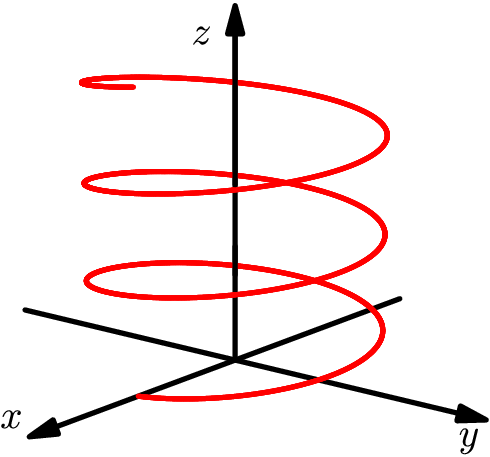
\includegraphics[scale=0.33]{Images/vectorValuedFunctions/Helix}
\end{figure}

\noindent
Since VVFs are essentially multiple single-input single-output functions packaged together, the domain of a VVF is the domain on which all components are defined.\\

\noindent
For example, if $\vec{r}(t) = \langle \tan{t},6t,\ln{\left(16-\right)} \rangle$,
\begin{itemize}
	\item $\tan{t}$ is defined for all real numbers equivalent to $\pm\pi/2$ radians.
	\item $6t$ is defined for all real numbers.
	\item $\ln{\left(16-t^2\right)}$ is defined for $t\in\left(-4,4\right)$.
\end{itemize}
The intersection of these domains is $\left(-4, -\pi/2\right) \cup \left(-\pi/2, \pi/2\right) \cup \left(\pi/2, 4\right)$, which is the domain of $\vec{r}(t)$.
\section{Derivatives of VVFs}
\noindent
Just like functions from Calc I and II, we can differentiate VVFs. In fact, the limit definitions of the derivative are nearly identical.\\
Let $\vec{r}(t) = \langle x(t), y(t), z(t) \rangle$.
\begin{align*}
	\vec{r^\prime}(t) &= \lim_{h\to 0}{\frac{\vec{r}(t+h)-\vec{r}(t)}{h}} \\
	&= \lim_{h\to 0}{\langle \frac{x(t+h)-x(t)}{h}, \frac{y(t+h)-y(t)}{h}, \frac{z(t+h)-z(t)}{h} \rangle}
\end{align*}
The limit distributes inside the vector, so
\begin{equation*}
	\vec{r^\prime}(t) = \langle x^{\prime}(t), y^{\prime}(t), z^{\prime}(t) \rangle
\end{equation*}

\noindent
Like a position function from Calc I and II, the derivative of a VVF representing position gives a VVF representing velocity, and the 2nd derivative gives a VVF representing acceleration. The magnitude of the velocity VVF, the speed, is commonly notated $v(t)$.\\

\noindent
There are 5 important properties of the derivatives of VVFs. These properties are similar to single-variable derivatives.\\
Let $\vec{r}(t)$ and $\vec{s}(t)$ be VVFs, $a(t)$ be a scalar function, and $c$ be a scalar.\\
\begin{enumerate}
	\item Linearity
	\begin{equation*}
		\frac{\mathrm{d}}{\mathrm{d}t}c\vec{r}(t) = c\vec{r^\prime}(t)	
	\end{equation*}
	\item Product Rule for Scalar Functions
	\begin{equation*}
		\frac{\mathrm{d}}{\mathrm{d}t}a(t)\vec{r}(t) = a(t)\vec{r^\prime}(t) + \vec{r}(t)a^{\prime}(t)
	\end{equation*}
	\item Dot Product Rule
	\begin{equation*}
		\frac{\mathrm{d}}{\mathrm{d}t}\vec{s}(t)\cdot\vec{r}(t) = \vec{s}(t)\cdot\vec{r^\prime}(t) + \vec{r}(t)\vec{s^\prime}(t)	
	\end{equation*}
	\item Cross Product Rule
	\begin{equation*}
		\frac{\mathrm{d}}{\mathrm{d}t}\vec{s}(t)\times\vec{r}(t) = \vec{s}(t)\times\vec{r^\prime}(t) + \vec{s^\prime}(t)\times\vec{r}(t)	
	\end{equation*}
	\item Chain Rule
	\begin{equation*}
		\frac{\mathrm{d}}{\mathrm{d}t}\vec{r}(a(t)) = \vec{r^\prime}(a(t))a^{\prime}(t)
	\end{equation*}
\end{enumerate}
A quotient rule doesn't make sense because we don't have an operation for dividing two vectors by each other.

\noindent
Just like in single variable calculus, we can use the derivative of VVFs to find tangent lines to the curve. Similar to how $f^{\prime}(a)$ represents the slope of $f$ at $a$, $\vec{r^\prime}(a)$ represents the direction of the tangent line at $a$. Remembering the VVF form of a line, the tangent line to $\vec{r}$ at $t$ is 
\begin{equation*}
	\vec{l}(t)=\vec{r}(t)+t\vec{r^\prime}(t)	
\end{equation*}
In fact, tangent lines appear so often, that we have a special unit vector representing the direction of the tangent line.
\begin{equation*}
	\hat{T}(t) = \frac{\vec{r^\prime}(t)}{\norm{\vec{r^\prime}(t)}}
\end{equation*}
You can remember $\hat{T}$ as the "tangent" vector.

\begin{figure}[H]
	\centering
	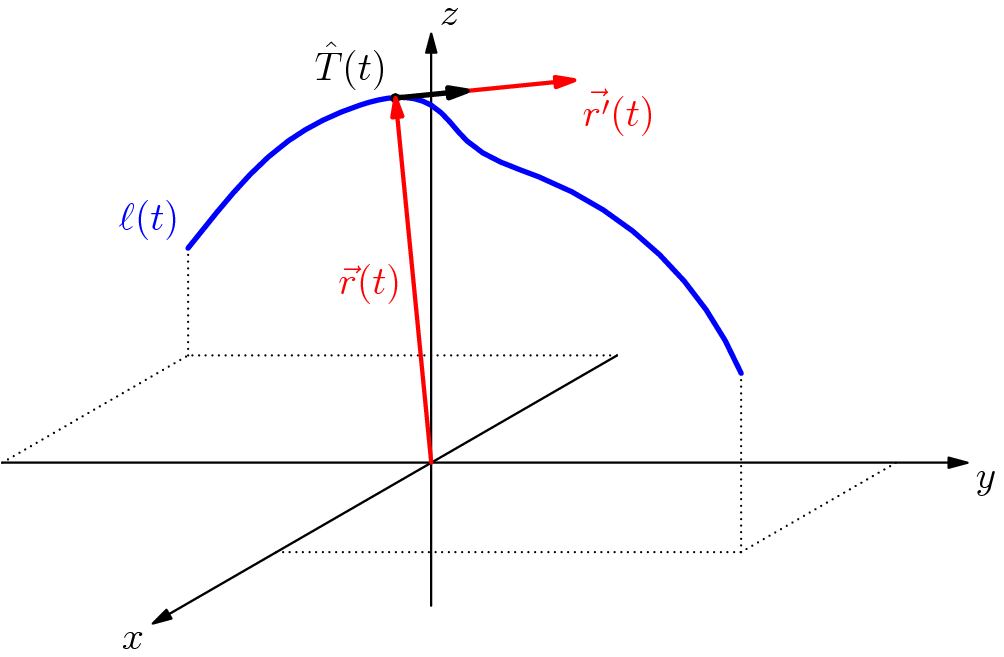
\includegraphics[scale=0.33]{Images/vectorValuedFunctions/TangentVector}
\end{figure}
\section{Integrals of VVFs}
VVFs can also be integrated. The integration operation also distributes inside the vector, for both definite and indefinite integrals.
$$\int{\vec{r}(t)\mathrm{d}t}=\left<\int{x(t)\mathrm{d}t},\int{y(t)\mathrm{d}t},\int{z(t)\mathrm{d}t}\right>$$
$\small{\text{Note: For indefinite integrals, the result will have a vector of constants will be added.}}$
\section{Reparameterization \& Arc Length}
\noindent
VVFs can be reparameterized to trace out the same curve at different speeds by replacing $t$ in $\vec{r}(t)$ with any non-decreasing function of $t$. This fact can come in handy to make the bounds of an integration problem more convenient.\\

\noindent
The integral of the derivative of a VVF gives the displacement vector because
\begin{equation*}
	\int_{a}^{b}{\vec{r^\prime}(t)\mathrm{d}t}=\vec{r}(b)-\vec{r}(a)
\end{equation*}
This is exactly like how velocity $\cdot$ time $=$ displacement.

\noindent
If we integrate the magnitude of $\vec{r^\prime}9t)$, we can use the fact that $\text{distance} = \text{speed}\cdot\text{time}$ to find the arc length of $\vec{r}(t)$ as
\begin{equation*}
	s=\int{\norm{\vec{r^\prime}(t)}\mathrm{d}t}=\int{\sqrt{\left(\frac{\mathrm{d}x}{\mathrm{d}t}\right)^2+\left(\frac{\mathrm{d}y}{\mathrm{d}t}\right)^2+\left(\frac{\mathrm{d}z}{\mathrm{d}t}\right)^2}\mathrm{d}t}
\end{equation*}
We can also write this as an arclength function,
\begin{equation*}
	s(t)=\int_{0}^{t}{\norm{\vec{r^{\prime}}(\tau)}\mathrm{d}\tau}
\end{equation*}

\noindent
If we have a function
\begin{equation*}
	f(t)=s(t)=\int_{0}^{t}{\norm{\vec{r^{\prime}}(\tau)}\mathrm{d}\tau}
\end{equation*}
where $s$ is strictly increasing, then $f$ has an inverse by the horizontal line test. That is $t(s) = f^{-1}(s)$ exists and is also non-decreasing. If we reparameterize $\vec{r}(t)$ to $\vec{r}(t(s))$, which is called the arc length parameterization, the parameterization will have a constant speed.
\section{TNB Frame \& Osculating Plane/Circle}
\subsection{T-Hat $\left(\hat{T}\right)$}
Arc length parameterization gives us another way to find $\hat{T}$.\\
\begin{equation*}
	\hat{T} = \frac{\vec{r^\prime}(t)}{\norm{\vec{r^\prime}(t)}} = \frac{\mathrm{d}\vec{r}/\mathrm{d}t}{\mathrm{d}s/\mathrm{d}t} = \frac{\mathrm{d}\vec{r}}{\mathrm{d}s}
\end{equation*}
\subsection{Curvature}
Curvature is 1 divided by the radius of the circle that best approximates the curve at a point. Tighter turns have smaller radii and higher curvature.\\
We can use $\hat{T}$ to find the curvature at a point on $\vec{r}(t)$.\\
\begin{equation*}
	\kappa(t) = \norm{\frac{\mathrm{d}\hat{T}}{\mathrm{d}s}} = \norm{\frac{\mathrm{d}\hat{T}}{\mathrm{d}t}\left(\frac{\mathrm{d}s}{\mathrm{d}t}\right)^{-1}} = \norm{\frac{\mathrm{d}\hat{T}}{\mathrm{d}t}}\frac{1}{v(t)}
\end{equation*}

\noindent
For example, let's find $\kappa(t)$ for the circle in the yz-plane: $\vec{r}(t)=\langle 7, R\sin{t}, R\cos{t} \rangle$.\\
\indent
$\vec{r^\prime}(t)=\langle 0, R\cos{t}, -R\sin{t}\rangle$ and $v(t)=\sqrt{0^2+(R\cos{t})^2+(-R\sin{t})^2}=R$\\
\indent
$\hat{T}(t)=\frac{1}{R}\vec{r}(t)=\langle0,\cos{t},-\sin{t}\rangle$, $\frac{\mathrm{d}\hat{T}}{\mathrm{d}t}=\langle 0,\sin{t},-\cos{t}\rangle$, $\norm{\frac{\mathrm{d}\hat{T}}{\mathrm{d}t}}=1$\\
\indent
$\kappa(t)=\frac{1}{R}$. This relationship is true for all circles.
\subsection{N-Hat $\left(\hat{N}\right)$}
\noindent
$\vec{r^{\prime}}(t) = v(t)\hat{T}(t)$\\
$\vec{r^{\prime\prime}}(t) = v(t)\hat{T}^{\prime}(t)+\hat{T}(t)v^{\prime}(t)$\\

\noindent
We will show that $\hat{T}(t) \perp \hat{T}^{\prime}(t)$.\\
\indent
$\frac{1}{2}\frac{\mathrm{d}}{\mathrm{d}t}\left(\hat{T}(t)\cdot\hat{T}(t)\right) = \hat{T}\cdot\hat{T}^{\prime}(t)$ and $\frac{\mathrm{d}}{\mathrm{d}t}\left(\hat{T}\cdot\hat{T}\right) = \frac{\mathrm{d}}{\mathrm{d}t}1 = 0$\\
\indent
So, $\hat{T}\cdot\hat{T}^{\prime}(t) = 0$ and $\hat{T}(t)\perp\hat{T}^{\prime}(t)$.\\
\noindent
\begin{equation*}
	\hat{N}(t)=\frac{\hat{T}^{\prime(t)}}{\norm{\hat{T}^{\prime}(t)}}\perp\hat{T}
\end{equation*}

\noindent
$\hat{N}$ is a unit vector perpendicular to $\hat{T}$ that points in the direction that the curve curls into. It is called the normal vector because it is perpendicular to the curve. It is in the same plane as $\vec{r}^\prime$, $\hat{T}$, and  $\vec{r}^{\prime\prime}$.

[INSERT IMAGE]

\noindent
$\hat{N}$ allows us to rewrite $\vec{r}^{\prime\prime}$.\\
\begin{equation*}
	\vec{r}^{\prime\prime}(t)=\frac{\mathrm{d}v}{\mathrm{d}t}\hat{T}(t)+v^{2}(t)\kappa(t)\hat{N}(t)
\end{equation*}

\noindent
We can see that $\vec{r}^{\prime\prime}(t)$ has two parts. If $\vec{r}(t)$ represents position, then $\frac{\mathrm{d}v}{\mathrm{d}t}$ represents linear acceleration and $v^2(t)\kappa(t)$ represents centripetal acceleration.\\ 
You might recognize the formula for centripetal acceleration in the 2nd part. If we let $R(t) = \frac{1}{\kappa(t)}$, then the 2nd part becomes $\frac{v^2(t)}{R(t)}$, which looks exactly like the formula for centripetal acceleration for uniform circular motion: $a_c = \frac{v^2}{r}$.
\subsection{Osculating Plane/Circle \& B-Hat $\left(\hat{B}\right)$}
\noindent
The osculating plane in the plane containing $\vec{r}(t)$, $\hat{T}$ and $\hat{N}$. It is only defined when $\hat{N}\neq 0$. This means strait lines do not have an osculating plane.\\

\noindent
The osculating circle lives in the osculating plane, is centered at $\vec{r}(t)+\frac{\hat{N}(t)}{\kappa(t)}$, and has radius $\frac{1}{\kappa(t)}$. The tangent line at $\vec{r}(t)$ is also tangent to the osculating circle because both points have the same curvature.

[INSERT IMAGES]

\noindent
The vector that is normal to the plane is $\hat{B}(t)=\hat{T}\times\hat{N}$, which is called the binormal vector because it is perpindicular to both $\hat{T}$ and $\hat{N}$. Together, $\hat{T}$, $\hat{N}$, and $\hat{B}$ form the Frenet Serret Frame, also called the TNB frame.

[INSERT IMAGES]

\noindent
We can write the equation for the osculating plane as $\hat{B}(t)\cdot\left(\langle x,y,z\rangle - \vec{r}(t)\right) =0$.
	\chapter{Differential Multivariable Calculus}
\section{Multivariable Functions}
\noindent
Multivariable functions take several values as an input and return a single value as an output.\\
For example, $ z =x^2 + y^2$ takes $\mathbb{R}^2 \to \mathrm{R}$.\\
Although we can only graph and fully visualize up to $\mathbb{R}^2 \to \mathbb{R}$ as a surface, we can imagine a multivariable function with 3 inputs ($\mathbb{R}^3 \to \mathbb{R}$) as a heatmap in 3D space. However, most of the mathematics we will discuss applies to functions with any number of inputs.\\

\noindent
The domain of a multivariable function $f: \mathbb{R}^n \to \mathbb{R}$ is the largest set of points on which $f$ is defined.\\
For example, if $f(x,y) = \ln{\left(9-x^2-y^2\right)}$, the domain of $f(x,y)$ is $\left\{ (x,y) | x^2+y^2<9 \right\}$.
\section{Level Curves}
\noindent
We can look at different cross sections of a surface $f(x,y)$ by looking at the equation $f(x,y)=c$ where $c\in\mathbb{R}$. This curve lives in the xy-plane and is called the C-level curve. We often visualize these curves in the $z=c$ plane as part of the surface. In higher dimensions, like $f(x,y,z)$, a C-level curve becomes a C-level surface.

[INSERT IMAGES]

\noindent
For example, the C-level surface of $f(x,y,z)=e^{-\left(x^2+y^2+z^2\right)}$ is the sphere centered at the origin with radius $\sqrt{-\ln{c}}$: $x^2+y^2+z^2=-\ln{c}$.
\section{Quadric Surfaces}
\noindent
Quadric surfaces extend parabolas and other shapes composed of at most squared terms into 3D.

\subsection{Paraboloids}
\noindent
The paraboloid looks like a parabola that has been rotated and extruded about its axis of symmetry.
It is radially symmetric, and its level curves are circles.
Paraboloids have the form $z = ax^2 + by^2$ where $a,b \in \mathbb{R}$.

\begin{figure}[H]
	\centering
	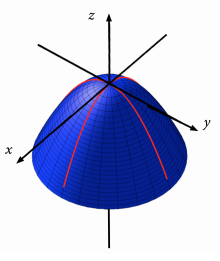
\includegraphics[width = 0.3\textwidth]{./Images/differentialMultivariableCalculus/paraboloid.png}
	\caption{A paraboloid}
\end{figure}
\subsection{Hyperboloids}
\noindent
A hyperboloid looks like a hyperbola that has been rotated and extruded about its center. It is also radially symmetric with circular level curves. Paraboloids have the form 
\begin{equation*}
	d = \pm \frac{x^2}{a^2} \pm \frac{y^2}{b^2} \pm \frac{z^2}{c^2},
\end{equation*}
where one sign is different from the others. Depending on the signs and the value of $d$, one can get a hyperboloid of one sheet, two sheets, or a cone.

\input{./differentialMultivariableCalculus/hyperboloidOneSheet}
\input{./differentialMultivariableCalculus/hyperboloidTwoSheet}
\input{./differentialMultivariableCalculus/cone}
\subsection{Hyperbolic Paraboloids}
\noindent
Hyperbolic paraboloids have the form $z = x^2 - y^2$. They are not radially symmetric and look like a saddle or Pringle's chip.

[INSERT IMAGE]
\subsection{Ellipsoids}
\noindent
Ellipsoids look like ellipses that have been rotated and extruded about their axis.
They are radially symmetric about this axis.
They have the general form 
\begin{equation*}
	d = \frac{x^2}{a^2} + \frac{y^2}{b^2} + \frac{z^2}{c^2}	
\end{equation*}
Note that the only difference in the equation between an ellipsoid and hyperboloid is the signs are all positive.

\begin{figure}[H]
	\centering
	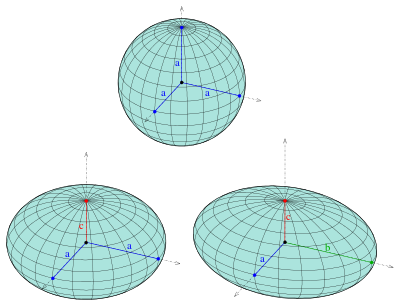
\includegraphics[width=0.66\textwidth]{./Images/differentialMultivariableCalculus/ellipsoids.png}
	\caption{Ellipsoids}
\end{figure}
\subsection{3D Cylinders}
\noindent
Although we normally think of cylinders as being extruded circles (circular cylinders), we can create other types of cylinders by extruding curves into 3D space.

\input{./differentialMultivariableCalculus/circularCylinder}
\input{./differentialMultivariableCalculus/parabolicCylinder}
\section{Parameterized Surfaces}
\noindent
Parameterized surfaces are a natural of VVFs that map $\mathbb{R}^n \to \mathbb{R}^m$ where usually $n<m$.\\

\noindent
For example, a cylinder of radius 1 can be parameterized as $\vec{r}(u,v) = \langle\sin{u}, \cos{u}, v\rangle$.
This particular surface maps $\mathbb{R}^2 \to \mathbb{R}^3$.
The paraboloid $z = x^2 + y^2$ can be parameterized as $\vec{r}(u,v)=\langle u, v, u^2+v^2 \rangle$.\\

\noindent
A general trick when trying to parameterize a surface is to substitute $u$ and $v$ for two variables like $x$ and $y$ and find an expression for the third variable in terms of the $u$ and $v$.
Although this does not always lead to the most useful parameterization, it can be a good starting point.\\

\noindent
For example, if we wanted to parameterize the surface $y^2=x^2+z^2$ from $y=1$ to $y=9$, we could use the general trick and get $\vec{r}(u,v) = \langle u,\sqrt{u^2+v^2},v\rangle$ where $1\leq u^2+v^2\leq 9^2$.
Although this parameterization is technically correct, it is difficult to work with because the bounds for $u$ and $v$ are not independent.\\
Instead, we can recognize that the surface we are trying to parameterize has radial symmetry about the $y$-axis and instead let $u$ be and angle and $v$ be a radius to get $\vec{r}(u,v) = \langle v\cos{u}, v, v\sin{u}\rangle$ where $0\leq u\leq 2\pi$ and $1\leq v\leq 9$.
The parameterization now has independent bounds, which will make operations like integration much easier.

\section{Limits \& Continuity in 3D}
\noindent
Limits in single-variable calculus are relatively simple because thera are only two ways to approach a point on a curve: left and right. When dealing with a surface, there are infinitely many ways to approach a point. So, we need a general and more formal idea of limits that works in higher dimensions.

\subsection{Open Delta Neighborhoods}
\noindent
An open delta neighborhood of a point $x_0$ is defined as the set
\begin{equation*}
	N\left(x_0, \delta\right) = \left\{x \in \mathbb{R}^n \mid \norm{x-x_0} < \delta\right\}.
\end{equation*}

\begin{figure}[H]
	\centering
	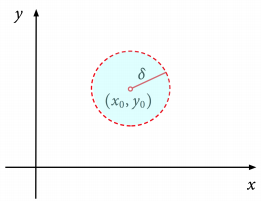
\includegraphics[width=0.5\textwidth]{./Images/differentialMultivariableCalculus/open_delta.png}
	\caption{An open delta neighborhood centered at $(x_0, y_0)$}
\end{figure}

\noindent
This simply means all points less than a distance $\delta$ away from point $x_0$.\\
For example, $N( (1,2) , 7) = \left\{ (x,y) \mid \sqrt{(x-1)^2 + (y-2)^2}<7 \right\}$, which is a ball (filled-in circle) of radius 7 centered at $(1, 2)$.
\subsection{Boundary Points, Open \& Closed Sets}
\noindent
Given some set $\Omega \subset \mathbb{R}^n$, $x$ is an interior point to $\Omega$ if $\exists \delta \mid N(x, \delta) \subset \Omega$. That is, $x$ is an interior point to $\Omega$ if you can draw a circle of non-zero radius around $x$ such that the entire circle is inside of $\Omega$.\\
All points that are not interior points are boundary points. Formally, $x$ is a boundary point of $\Omega$ if $\forall \delta \mid N(x,\delta) \not\subset \Omega$.\\
Using our definitions of interior and boundary points, we can define and open set as one that doesn't contain any of its boundary points and a closed set as one that contains all of its boundary point. Note that a set that contains some of its boundary points is neither open nor closed.
\subsection{Limit \& Continuity Definitions}
\noindent
Finally, we have the proper tools to define a limit in higher dimensions. We say that $\lim_{p\to p_0}f(p) = L$ if $\forall N(L\epsilon)$, $\exists N(p_0,\delta) \mid p \in N(p_0, \delta) \implies f(p) \in N(L, \epsilon)$.\\
That is, the limit of $f(p)$ as $p$ approaches $p_0$ is equal to $L$ if for all open delta neighborhoods around $L$, there exists an open delta neighborhood around $p_0$ such that $p$ being in the neighborhood around $p_0$ means $f(p)$ must be in the neighborhood around $L$.

[INSERT IMAGE]

\noindent
Now with a limit definition, we can define continuity at a point. We say that a function $f : \mathbb{R}^n \to \mathbb{R}$ is continuous at $p_0$ if $\lim_{p \to p_0}{f(p)} = f(p_0)$.\\

\noindent
\begin{theorem}
	Trigonometric functions, exponentials, logarithms, and sums, products, quotients, and compositions of such functions are continuous on their domain.
\end{theorem}

\noindent
Although our definitions allow us to confirm that a value is the limit of a function, they do not give us any insight into how to find the value of the limit. We'd need to approach our point of interest from every possible direction to see if the limit from that direction is the same as all the others. If any two directions give different limit values, then the limit doesn't exist.\\
We approach a function, $f$, by composing it with a single variable path, $\vec{r}(t)$, that goes through the point of interest, and find the limit along the path.\\

\noindent
If $f$ is some surface $f(x, y)$ and $\vec{r}(t) = \langle x(t), y(t)\rangle$, then the composition of $f$ and $\vec{r}$ is $f\circ\vec{r} = f(\vec{r}(t)) = f(x(t), y(t))$.\\
For example, let's try to find
\begin{equation*}
	\lim_{(x,y) \to (0,0)}{\frac{x^2-y^3}{x^2+y^2}}
\end{equation*}
\indent
We'll choose two paths $\vec{r_1}(t) = \langle t, 0 \rangle$ and $\vec{r_2}(t) = \langle t, t \rangle$ and find the limit as $t \to 0$ in both cases.\\
\indent
\begin{equation*}
	\lim_{t \to 0}{f(\vec{r_1}(t))} = \lim_{t \to 0}{\frac{t^2}{t^2}} = 1
\end{equation*}
\indent
\begin{equation*}
	\lim_{t \to 0}{f(\vec{r_2}(t))} = \lim{t \to 0}{\frac{t^2-t^3}{2t^2}} = \lim_{t \to 0}{\frac{1}{2} - \frac{t}{2}} = \frac{1}{2}
\end{equation*}
\indent
Since the limits on the two paths are not equal, we can say that
\begin{equation*}
	\lim_{(x,y) \to (0,0)}{\frac{x^2-y^3}{x^2+y^2}} = \text{ DNE}
\end{equation*}
\section{Partial Derivatives}
\noindent
The single-variable calculus idea of tangent lines doesn't work for higher dimensional surfaces because we can draw many different lines that are tangent to the surface, depending on which plane we use to slice the surface. That is, from which direction we approach the surface.
\subsection{Partial Derivatives of X, Y, and Z}
\noindent
It's common to look at the derivative when slicing a surface in the yz, xz, and xy planes. These are called partial derivatives.\\

\noindent
To compute $\frac{\partial}{\partial x}{f(x,y)}$, we take the derivative with respect to $x$ as if $y$ is constant. Formally,
\begin{equation*}
	\frac{\partial}{\partial x}f(x,y) = \lim_{h \to 0}{\frac{f(x+h,y)-f(x,y)}{h}}
\end{equation*} 
and 
\begin{equation*}
	\frac{\partial}{\partial y}f(x,y) = \lim_{h \to 0}{\frac{f(x,y+h)-f(x,y)}{h}}
\end{equation*}

\noindent
We also use the shorthand $\frac{\partial}{\partial x}=f_x$ and $\frac{\partial}{\partial y}=f_y$. This shorthand can be extended to higher-order derivatives so that $\frac{\partial}{\partial y}\left(\frac{\partial}{\partial x}f(x,y)\right)=f_{xy}$.

\noindent
Fubini's Theorem (also called Tonelli's or Clairaut's Theorem) says $f_{xy} = f_{yx}$, $f_{xz} = f_{zx}$, and $f_{yz} = f_{zy}$. It extends into higher-order mixed partial derivatives, saying that two mixed partial derivatives of a function are equal as long as they both differentiate the same number of variables the same number of times. So, $f_{abcdab} = f_{aacdbb}$.
\subsection{Tangent Planes}
\noindent
Although the tangent lines at a point on a surface can all be different depending on from which direction one approaches a point, all of these tangent lines lie in the same plane, defining the tangent plane.
This means that the tangent plane to $z = f(x, y)$ at $(x_0,y_0)$ has the following properties:
\begin{itemize}
	\item The z-value of the tangent plane at $(x_0, y_0)$ is the same as $f(x_0, y_0)$.
	\item The value of the first-order partial derivatives of the tangent plane at $(x_0, y_0)$ should match those of $f(x_0, y_0)$.
\end{itemize}

\noindent
The general form of a plane at $(x_0, y_0, z_0)$ is
\begin{equation*}
	P(x,y) = A(x-x_0) + B(y-y_0) + z_0.
\end{equation*}
We want $P_x = f_x$ and $P_y = f_y$.
This means that $P_x = f_x = A$ and $P_y = f_y = B$.
Rewriting,
\begin{equation*}
	P(x,y) = f_x(x-x0) + f_y(y-y_0) + z_0.
\end{equation*} 
The normal vector is $\langle \pm f_x,\pm f_y, \mp 1\rangle$.
So, the point normal form of the plane is 
\begin{equation*}
	\langle -f_x, -f_y, 1\rangle \cdot \langle x-x_0, y-y_0, z-f(x_0,y_0) \rangle = 0.
\end{equation*}

\begin{figure}[H]
	\centering
	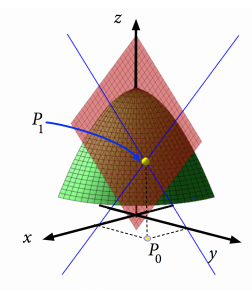
\includegraphics[width=0.5\textwidth]{./Images/differentialMultivariableCalculus/tangent_plane.png}
	\caption{Tangent plane}
\end{figure}

\subsection{Linear Approximations}
\noindent
Since $\partial z = f_x\partial x + f_y\partial y$, we can approximate $\Delta z$ (the change in any function) as $\Delta z \approx f_x\Delta x + f_y\Delta y$, since values of $f$ and the tangent plane are close. We an rewrite this approximation as a dot product: $\Delta z \approx \langle f_x, f_y\rangle \cdot \langle \Delta x, \Delta y \rangle$.\\

For example, say a cylindrical can has a radius $r=1$ and a height $h=5$. If the radius is increased by .1 and the height is increased by 1, what is the approximate $\Delta V$?
\begin{equation*}
	V(r,h) = \pi r^2 h, V_r = 2\pi rh \text{, and } V_h = \pi r^2
\end{equation*}
\begin{equation*}
	V_{r}(1,5) = 10\pi  \text{ and } V_{h}(1,5) = \pi
\end{equation*}
\begin{equation*}
	\Delta V \approx 10\pi(.1) + \pi(1) = 2\pi	
\end{equation*}
Comparing this to the actual answer of $2.26\pi$, we see our approximation is decent.
\section{The Gradient}
\noindent
If you have a surface $f:\mathbb{R}^2\to\mathbb{R}$, what direction $\langle \Delta x, \Delta y\rangle$ should I go to maximize the change if $f$?\\
We saw earlier that $\Delta z\approx \langle f_x,f_y\rangle\cdot\langle\Delta x, \Delta y\rangle$. To maximize a dot product, $\langle \Delta x, \Delta y\rangle$ should be in the same direction as $\langle f_x, f_y\rangle$. This directional vector is called the gradient: the direction of steepest ascent.\\
Notated mathematically, $\nabla f(x,y) = \langle f_x, f_y\rangle$.

[INSERT IMAGE]

\subsection{Gradient Properties}
\noindent
Let $f$ and $g$ be functions of multiple variables, let $\vec{r}$ be a VVF, and let $c\in\mathbb{R}$.
\begin{enumerate}
	\item $\nabla(f\pm g)=\nabla f\pm\nabla g$
	\item $\nabla(cf)=c\nabla f$
	\item $\nabla(fg)=f\nabla g+g\nabla f$
	\item $\nabla(f\circ\vec{r}(t))=\nabla f\cdot\vec{r}(t)$
\end{enumerate}
\subsection{Linear Approximations with the Gradient}
\noindent
We can rewrite our linear approximation of $f$ at $x_0$ using the gradient.
\begin{equation*}
	f(x) \approx f(x_0) + (\nabla f)(x_0) \cdot (x - x_0)
\end{equation*}
\subsection{The Gradient \& C-Level Curves}
\noindent
Let $\vec{r}(t)$ be the C-level curve of $f(x, y)$.
\begin{align*}
f\circ\vec{r} &= C  \text{ and } \frac{\mathrm{d}}{\mathrm{d}t}(f\circ\vec{r}) = 0 \\
	&\implies \frac{\mathrm{d}}{\mathrm{d}t}(f\circ\vec{r}) = \nabla f\cdot\vec{r^\prime}(t) = 0 \\
	&\implies \nabla f\perp\vec{r^\prime}(t) \\
	&\implies \nabla f \text{ is perpendicular to the C-level curve of } f.
\end{align*}

[INSERT IMAGE]
\section{Directional Derivatives}
\noindent
We already saw partial derivatives in the $x$, $y$, and $z$ directions.
However, we can take the derivative coming from other directions.
These are called directional derivatives, $D_{\hat{u}}{f}$, where $\hat{u}$ is the direction.
\begin{equation*}
	D_{\hat{u}}{f} = \lim_{h \to 0}{\frac{f(\vec{p_0} + h\hat{u})}{h}}
\end{equation*}
\noindent
If $\hat{u} = \langle a, b \rangle$, 
\begin{equation*}
	D_{\hat{u}}{f} = \lim_{h \to 0}{\frac{f(x+ah, y+bh) - f(x,y)}{h}}	
\end{equation*}
Note that
\begin{equation*}
	D_{\hat{i}}{f} = \lim_{h \to 0}{\frac{f(x+h, y) - f(x, y)}{h}} = f_x \text{ and } D_{\hat{j}}{f} = f_y	
\end{equation*}
Let's look at $D_{\hat{u}}{f}$.
\begin{align*}
	D_{\hat{u}}{f} &= \lim_{h \to 0}{\frac{f(x+ah, y+bh) - f(x+ah, y) + f(x+ah, y) - f(x, y)}{h}} \\
	&= b\lim_{h \to 0}{\frac{f(x+ah, y+bh)-f(x+ah, y)}{bh}} + a\lim_{h \to 0}{\frac{f(x+ah, y) - f(x, y)}{ah}} \\
	&= b\frac{\partial f}{\partial y} + a\frac{\partial f}{\partial x} \\
	&= af_x + bf_y
\end{align*}
So, 
\begin{equation*}
	D_{\hat{u}}{f} =\nabla f \cdot \hat{u}.
\end{equation*}

\section{Optimization}
\subsection{Definitions}
\begin{enumerate}
	\item $f(x_0, y_0)$ is a local maximum of $f$ if for some $\delta > 0$, $f(x_0, y_0) \geq f(x, y) \forall (x,y) \in N((x,y),\delta)$.
		That is, you can draw a circle in the domain of $f$ centered at $(x_0, y_0)$ such that the value of $f$ at every point in the circle besides $(x_0, y_0)$ is less than $(x_0, y_0)$.
	\item $f(x_0, y_0)$ is a local minimum of $f$ if for some $\delta > 0$, $f(x_0, y_0) \leq f(x,y) \forall (x,y) \in N((x,y),\delta)$.
		That is, you can draw a circle in the domain of $f$ centered at $(x_0, y_0)$ such that the value of $f$ at every point in the circle besides $(x_0, y_0)$ is greater than $(x_0, y_0)$.
	\item $f(x_0, y_0)$ is a global max of $f$ if $f(x_0, y_0) \geq f(x,y) \forall (x,y) \in D(f)$ where $D(f)$ is the domain of $f$.
	\item $f(x_0, y_0)$ is a global min of $f$ if $f(x_0, y_0) \leq f(x,y) \forall (x,y) \in D(f)$ where $D(f)$ is the domain of $f$.
\end{enumerate}
\begin{theorem}
	If $(x_0, y_0)$ is in the domain of $f$ and a local extrema of $f(x,y)$, then $f_x(x_0, y_0)$ and $f_y(x_0, y_0)$ is either 0 or undefined.
\end{theorem}

\begin{figure}[H]
	\centering
	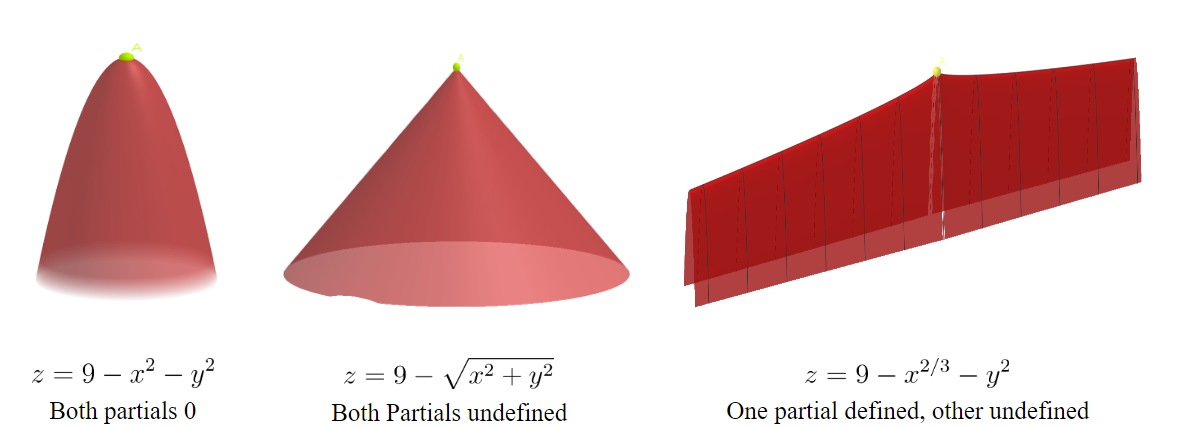
\includegraphics[width=0.9\textwidth]{./Images/differentialMultivariableCalculus/optimization.png}
	\caption{Critical points appear when the partial derivatives are 0 or undefined.}
\end{figure}
\subsection{Critical Points}
\noindent
Critical points are those that have the possibility of being a minimum or maximum. They are an extension of critical points in single-variable calculus when the derivative is 0.\\

\noindent
\begin{definition}
	$(x_0, y_0)$ is a critical point of $f$ if $f_x$ and $f_y$ at $(x_0, y_0)$ both are 0 or DNE.
\end{definition}

\noindent
For example, consider the function $f(x,y) = x^2/2 - y^2/2 - xy - 2x - 2y$.
\begin{equation*}
	f_x = x - y - 2	\text{ and is } 0 \text{ when } y = x-2
\end{equation*}
\begin{equation*}
	f_y = -y - x - 2 \text{ and is } 0 \text{ when } y = -x-2
\end{equation*}
\begin{equation*}
	x - 2 = -x -2 \text{ when } x = 0
\end{equation*}
When $x = 0$, $ y =-2 \implies (0, -2)$ is a critical point of $f$.

\input{./differentialMultivariableCalculus/2ndDerivativeTestHessianMatrix}
\subsection{Gradient Descent}
\noindent
Remember that if we have a multidimensional function, taking a step in the direction of the gradient results in the maximum possible increase of the function, and taking a step in the opposite direction of the gradient results in the maximum possible decrease of the function. Gradient descent is a method to find minima of functions.\\

\noindent
Let's say we're trying to minimize $J(\vec{x})$ with gradient descent. Here are the steps we would take:
\begin{enumerate}
	\item Pick (or guess) a starting point $\vec{x_0}$ and a learning rate (step size) $\delta$.
	\item $\vec{x_{n+1}}=\vec{x_n}-\delta J(\vec{x_n})$
	\item Repeat step 2 until some stopping criteria is met, like $\norm{\delta\nabla J(\vec{x_n})-\delta\nabla J(\vec{x_{n+1}})}<.01$.
\end{enumerate}

[INSERT IMAGE]

\noindent
This method will lead you arbitrarily close to a local minimum, but does not guarantee finding the global minimum. More advanced versions of gradient descent exists that try to help with this, like giving the point “momentum” to be able to move out of local mins.
This method also has a tradeoff between speed and accuracy. Although increasing $\delta$ means fewer iterations of gradient descent are needed to narrow in on a local minimum, one is more likely to be stuck in a local min than they had used a smaller $\delta$.\\

\noindent
In the real world, the function you are trying to minimize will likely not be well defined enough to take its partial derivatives to find the gradient, so they too are approximated by doing something like $$J_{k}=\frac{J(k+.0001,...)-J(k,...)}{.0001}$$
\subsection{Lagrange Multipliers}
\noindent
Lagrange multipliers are a method that allow us to find extrema of a function subject to domain constraints.\\

\input{./differentialMultivariableCalculus/toyExample}

\noindent
In the example above, $f_x = 1$, $g_x = 2x$, $f_y = 1$, and $g_y = 2y$ with constraint $x^2 + y^2 = 1$.\\ 
Giving us a system
\begin{equation*}
	\begin{cases}
		1 = \lambda 2x \\ 
		1 = \lambda 2y \\ 
		x^2 + y^2 = 1
	\end{cases} \implies x = y = \pm \frac{1}{\sqrt{2}}\text{ and } \lambda = \frac{1}{\sqrt{2}}
\end{equation*}
This means that the max value of $f$ constrained by $g$ is
\begin{equation*}
	f\left(\frac{1}{\sqrt{2}},\frac{1}{\sqrt{2}}\right) = \sqrt{2}
\end{equation*}

\input{./differentialMultivariableCalculus/methodLagrangeMultipliers}
	\chapter{Multiple Integrals}
\section{Double Integrals}
\noindent
Similar to how the limit of a Riemann Sum, the sum of the areas of small rectangles, is the area underneath a curve, we can find the volume underneath a surface by summing the volumes of small rectangular prisms.\\

[INSERT IMAGE]

\noindent
In 2D (single variabe): $\Delta x = \frac{b-a}{n}$, $\int_{a}^{b}{f(x)\mathrm{d}x} = \lim_{n \to \infty}{\sum_{i = 0}^{n-1}{f(a+i\Delta x)\Delta a}}$.\\
In 3D: $\Delta x = \frac{b-a}{n}$, $\Delta y = \frac{d-c}{n}$,
\begin{equation*}
	\int_{c}^{d}{\int_{a}^{b}{f(x,y)\mathrm{d}x}\mathrm{d}y} = \lim_{m \to \infty}{\sum_{j = 0}^{m-1}{\left(\lim_{n \to \infty}{\sum_{i = 0}^{n-1}{f(a+i\Delta a, c+j\Delta y)\Delta x}}\right)\Delta y}}
\end{equation*}
\subsection{Fubini's Theorem \& Domain Regions}
\begin{theorem}[Fubini's Theorem]
	The order of integration on a domain where the variables of integration $\left(x, y, \text{etc.}\right)$ vary independently doesn't matter.
\end{theorem}

\noindent
For example, let's find the volume under $f(x,y) = 9-x^2-y^2$, $(x,y) \in [0,1] \times [1,2]$.\\
We will do so in two ways to show that they are equivalent: one with $x$ first and then $y$ and another with $y$ first and then $x$.\\
\begin{center}
	\begin{tabular}{c|c}
		$V = \int_{0}^{1}{\int_{1}^{2}{9 - x^2 - y^2\mathrm{d}y}\mathrm{d}x}$ & $V =\int_{2}^{1}{\int_{0}^{1}{9 - x^2 - y^2\mathrm{d}x}\mathrm{d}y}$ \\
		$= \int_{0}^{1}{\left[9y - x^2y - \frac{y^2}{3}\right]_{1}^{2}\mathrm{d}x}$ & $= \int_{1}^{2}{\left[9x - \frac{x^3}{3} - xy^2\right]_{0}^{1}\mathrm{d}y}$ \\
		$= \int_{0}^{1}{\frac{20}{3} - x^2\mathrm{d}x}$ & $= \int_{1}^{2}{\frac{26}{3} - y^2\mathrm{d}y}$ \\
		$= \left[\frac{20}{3}x - \frac{x^3}{3}\right]_{0}^{1}$ & $= \left[\frac{26}{3}y - \frac{y^3}{3}\right]_{1}^{2}$ \\
		$= \frac{19}{3}$ & $= \frac{19}{3}$ \\
	\end{tabular}
\end{center}

\noindent
Let's look at a case where $x$ and $y$ are not independent. specifically, where the bounds on $y$ are a function of $x$.

[INSERT IMAGE]

\noindent
This is called a Type I Region. Formally, a Type I Region is a domain $D = \left\{ (x,y) \mid a \leq x \leq b, g(x) \leq y \leq h(x) \right\}$.\\

\begin{theorem}[Fubini's Theorem for Type I Regions]
	Let $D$ be a Type I Region in $\mathbb{R}^2$.\\
	\begin{equation*}
		\iint\limits_{D}{f(x,y)\mathrm{d}A} = \int_{a}^{b}{\int_{g(x)}^{h(x)}{f(x,y)\mathrm{d}y}\mathrm{d}x}
	\end{equation*}
\end{theorem}

\noindent
It's also possible for y to have constant bounds and the bound for $x$ to be a function of $y$. this is a Type II Region. Formally, a Type II Region is a domain $D = \left\{(x,y) \mid g(y) \leq x \leq h(y), a \leq y \leq b\right\}$.

\begin{theorem}[Fubini's Theorem for Type II Regions]
	Let $D$ be a Type II Region in $\mathbb{R}^2$.
	\begin{equation*}
		\iint\limits_{D}{f(x,y)\mathrm{d}A} = \int_{a}^{b}{\int_{g(y)}^{h(y)}{f(x,y)\mathrm{d}x}\mathrm{d}y}
	\end{equation*}
\end{theorem}

\noindent
Sometimes, a region can be describes as both Type I and Type II. You should pick whichever description is most convenient.\\

\noindent
The previous two theorems can be summarized as dependent variables need to be integrated before the variables that they depend on. This core idea extends into higher dimensions where classifying regions becomes tedious and not very helpful.\\

\noindent
One can split larger, harder to describe domains into smaller domains. Let $D_1 \cup D_2 = D$.

[INSERT IMAGE]

\begin{equation*}
	\iint\limits_{D}{f(x,y)\mathrm{d}A} = \iint\limits_{D_1}{f(x,y)\mathrm{d}A} + \iint\limits_{D_2}{f(x,y)\mathrm{d}A} - \iint\limits_{D_1 \cap D_2}{f(x,y)\mathrm{d}A}
\end{equation*}
\subsection{Average Values}
\noindent
We can think of the average value of a function over some interval as the answer to the question: “If I flattened this function into a box over the interval, what would the height of the box be?”\\
For single-variable functions, the answer is $\bar{f}=\frac{1}{b-a}\int_{a}^{b}{f(x)\mathrm{d}x}=\frac{\int_{a}^{b}{f(x)\mathrm{d}x}}{\int_{a}^{b}{\mathrm{d}x}}$.\\
This idea of summing a function over a domain and the dividing by the size of that domain holds into multivariable as
$$\bar{f}=\frac{\int\limits_{D}{f(x,y)\mathrm{d}D}}{\int\limits_{D}{\mathrm{d}D}}$$

\input{./multipleIntegrals/meanValueTheorem}
\subsection{Volume Between Surfaces}
\noindent
Similar to how we could find the area between two curves in single-variable calculus, we can find the volume between two surfaces.
\begin{equation*}
	V_{\text{bwtn}} = \iint\limits_{D}{f\mathrm{d}A} - \iint\limits_{D}{g\mathrm{d}A} = \iint\limits_{D}{(f-g)\mathrm{d}A}
\end{equation*}

\noindent
If $g$ is below $f$ in $D_1 \subset D$ but is above $f$ in $D_2 \subset D$, where $D_1 \cup D_2 = D \text{ and } D_1 \cap D_2 = \emptyset$, we can still find the volume between the surfaces by splitting $D$ into $D_1$ and $D_2$.
\begin{equation*}
	V_{\text{bwtn}} = \iint\limits_{D}{\abs{f-g}\mathrm{d}A} = \iint\limits_{D_1}{(f-g)\mathrm{d}A} + \iint\limits_{D_2}{(g-f)\mathrm{d}A}
\end{equation*}
\subsection{Plane Laminas}
\begin{definition}
	A plane lamina is an idealized 2D (0 thickness) object with mass that occupies a region $D \subset \mathbb{R}^2$.
\end{definition}

\noindent
Some questions one may ask about a plane lamina are ``What is the total mass?'' and ``Where is the center of mass?''.\\
We can think of the mass as 
\begin{equation*}
	M = \iint\limits_{D}{\sigma(x,y)\mathrm{d}A}
\end{equation*}
where $\sigma(x,y)$ is the mass density of the lamina at $(x,y)$.\\
The center of mass is
\begin{equation*}
	\bar{x} = \frac{M_y}{M} = \frac{\iint\limits_{D}{x\sigma(x,y)\mathrm{d}A}}{M} \text{ and } \bar{y} = \frac{M_x}{M} = \frac{\iint\limits_{D}{y\sigma(x,y)\mathrm{d}A}}{M}
\end{equation*}
where $M_x$ is the moment about the $x$-axis and $M_y$ is the moment about the $y$-axis.
\section{Triple Integrals}
\noindent
Triple integrals work much the same way as single and double integrals. They are still defined by a Riemann sum, and Fubini’s theorems about independent domains and the order of integration still applies.

\subsection{Fubini's Theorem for Z-simple Regions}
\noindent
There is another case of Fubini’s Theorem that arises in 3D.\\
\begin{theorem}[Fubini's Theorem for Z-simple Regions]
	Let $D\subset\mathbb{R}^3$ and let $\Omega=\left\{(x,y,z)|(x,y)\in D, g(x,y)\leq z\leq h(x,y)\right\}$ be a z-simple region.\\
	$$\iiint\limits_{\Omega}{f(x,y,z)\mathrm{d}V}=\iint\limits_{D}{\int_{g(x,y)}^{h(x,y)}{f(x,y,z)\mathrm{d}z}\mathrm{d}A}$$
\end{theorem}

\noindent
In other words, dependent variables must be integrated before the independent variables on which they rely, but the order of integration of independent variables doesn't matter.\\

\noindent
For example, we an express the unit sphere as a z-simple region where $D=\left\{(x,y)|x^2+y^2\leq 1\right\}$ and $-\sqrt{1-x^2-y^2}\leq z\leq\sqrt{1-x^2-y^2}$. Note that $D$ is a Type I Region.\\
$$V_{\text{sphere}}=\int_{-1}^{1}{\int_{-\sqrt{1-x^2}}^{\sqrt{1-x^2}}{\int_{-\sqrt{1-x^2-y^2}}^{\sqrt{1-x^2-y^2}}{\mathrm{d}z}\mathrm{d}x}\mathrm{d}x}=\frac{4\pi}{3}$$
\subsection{Laminas}
\noindent
Similar to plane laminas:
\begin{equation*}
	M = \iiint\limits_{\Omega}{\sigma(x,y,z)\mathrm{d}V}
\end{equation*}
\begin{tabular}{ccc}
	$\bar{x} = \frac{M_{yz}}{M} = \frac{\iiint\limits_{\Omega}{x\sigma(x,y,z)\mathrm{d}V}}{M}$ & $\bar{y} = \frac{M_{xz}}{M} = \frac{\iiint\limits_{\Omega}{y\sigma(x,y,z)\mathrm{d}V}}{M}$ & $\bar{z} = \frac{M_{xy}}{M} = \frac{\iiint\limits_{\Omega}{z\sigma(x,y,z)\mathrm{d}V}}{M}$ \\
\end{tabular}
	\chapter{Curvilinear Coordinates}
\noindent
You should already know about Cartesian $(x,y)$ coordinates and polar $(r,\theta)$ coordinates in 2D. Cartesian extends to 3D as $(x,y,z)$, but there are multiple ways to extend polar coordinates into 3D.\\

\section{Review of Polar Coordinates}
\noindent
Polar coordinates represent every point in 2D space as a distance from the origin $r$ and an angle from the horizontal $\theta$. This means that unlike rectangular (Cartesian) $(x,y)$ coordinates, different polar coordinates can represent the same point: $(2,-\pi/4)=(-2,3\pi/4)=(2,7\pi/4)$.

[INSERT IMAGE]

\noindent
Polar coordinates can be transformed into rectangular coordinates by $x=r\cos{\theta}$ and $y=r\sin{\theta}$. this means that $r=\sqrt{x^2+y^2}$ and $\theta=\tan^{-1}{\frac{y}{x}}$.

\subsection{Circles}
\noindent
A circle of radius $R$ centered at the origin can be represented as $r = R$.\\
Circles not centered at the origin require using the transformation equations.
\begin{equation*}
	(x-a)^2 + (y-b)^2 = R^2 \implies (r\cos{\theta}-a)^2 + (r\sin{\theta}-b)^2 = R^2
\end{equation*}
\begin{equation*}
	r^2\cos^{2}{\theta} + r^2\sin^{2}{\theta} - 2ra\cos{\theta} - 2rb\sin{\theta} + a^2 + b^2 = R^2
\end{equation*}
\begin{equation*}
	r^2 - 2r(a\cos{\theta} + b\sin{\theta}) - R^2 + a^2 + b^2 = 0
\end{equation*}
\begin{equation*}
	r = (a\cos{\theta} + b\sin{\theta}) \pm \sqrt{R^2 - a^2 - b^2 + (a\cos{\theta} + b\sin{\theta})^2}
\end{equation*}
\subsection{Lines}
\begin{itemize}
	\item Lines through the origin can be represented as $\theta = \tan^{-1}{m}$ where $m$ is the slope of the line.
	\item Lines of the form $x = a$ can be represented as $r = a\sec{\theta}$.
	\item Lines of the form $y = a$ can be represented as $r = a\csc{\theta}$.
	\item All other lines of the form $y=ax+b$ can be represented as $r = \frac{b}{\sin{\theta} - a\cos{\theta}}$. This form also covers the previous 2.
\end{itemize}
\subsection{Integration}
\noindent
The line element is $\mathrm{d}s^2=\mathrm{d}r^2+r^2\mathrm{d}\theta^2$, meaning that $s=\int_{\theta_1}^{\theta_2}{\sqrt{r^2+\left(\frac{\mathrm{d}r}{\mathrm{d}\theta}\right)}\mathrm{d}\theta}$.\\
The area element is $\mathrm{d}A=r\mathrm{d}r\mathrm{d}\theta$, meaning that $A=\int_{\theta_1}^{\theta_2}{r^2\mathrm{d}\theta}$.

\input{./curvilinearCoordinates/gaussianIntegral}
\section{Cylindrical Coordinates}
\noindent
Cylindrical coordinates are the expansion of polar coordinates by including a third term that represents the height from the xy-plane, $z$. All cylindrical coordinates have the form $(r,\theta,z)$. This system is called cylindrical because it’s easy to describe shapes with cylindrical symmetry because integrations have constant, independent bounds.

[INSERT IMAGE]

\subsection{Conversions}
\noindent
From Cylindrical to Cartesian: $(r,\theta,z)=(r\cos{\theta},r\sin{\theta},z)$\\
From Cartesian to Cylindrical: $(x,y,z)=\left(\sqrt{x^2+y^2},\tan^{-1}{\frac{y}{x}},z\right)$\\

\subsection{Integration}
\noindent
The volume element in cylindrical coordinates is $\mathrm{d}V=r\mathrm{d}r\mathrm{d}\theta\mathrm{d}z$.

[INSERT IMAGE]

\noindent
For example, let's evaluate $\int_{0}^{4}{\int_{0}^{\sqrt{16-y^2}}{\int_{0}^{16-x^2-y^2}{\mathrm{d}z}\mathrm{d}x}\mathrm{d}y}$, the volume under the paraboloid $z=16-x^2-y^2$ using cylindrical coordinates.\\
\indent
$=\int_{0}^{4}{\int_{0}^{\pi/2}{\int_{0}^{16-r^2}{r\mathrm{d}z}\mathrm{d}\theta}\mathrm{d}r}$\\
\indent
$=\int_{0}^{4}{\int_{0}^{\pi/2}{16r-r^2\mathrm{d}\theta}\mathrm{d}r}$\\
\indent
$=\frac{\pi}{2}\int_{0}^{4}{16r-r^3\mathrm{d}r}$\\
\indent
$=\frac{\pi}{2}\left[8r^2-\frac{r^4}{4}\right]_0^4$\\
\indent
$=32\pi$\\

\noindent
For another example, let's find the average value of $f(x,y,z)=z$ on the domain $\Omega$ which is bounded by $z=\sqrt{6-x^2-y^2}$ and $z=x^2+y^2$.\\
\indent
$\bar{f}=\frac{\int_{0}^{2\pi}{\int_{0}^{\sqrt{2}}{\int_{r^2}^{\sqrt{6-r^2}}{zr\mathrm{d}z}\mathrm{d}r}\mathrm{d\theta}}}{\int_{0}^{2\pi}{\int_{0}^{\sqrt{2}}{\int_{r^2}^{\sqrt{6-r^2}}{r\mathrm{d}z}\mathrm{d}r}\mathrm{d}\theta}}=\frac{11}{12\sqrt{6}-17}$\\
\indent
$\small{\text{Work omitted for brevity}}$\\
\section{Spherical Coordinates}
\noindent
Unlike how cylindrical coordinates extend polar coordinates into 3D by adding a Cartesian term, spherical coordinates add an angular term, $\phi$, the azimuthal angle. All spherical coordinates have the form $(\rho,\theta,\phi)$ where $\rho$ is the distance from the origin, $\theta$ is the polar angle in the xy-plane, and $\phi$ is the azimuthal angle from the $+z$-axis. Shapes with spherical symmetry have a constant bounds of integration in spherical coordinates.

[INSERT IMAGE]

\subsection{Conversions}
\noindent
From spherical to Cartesian: $(\rho, \theta, \phi) = (r\cos{\theta}\sin{\phi}, \rho\sin{\theta}\sin{\phi}, \rho\cos{\phi})$\\
From Cartesian to Spherical: $(x, y, z)=\left(\sqrt{x^2 + y^2 + z^2}, \tan^{-1}{\left(\frac{y}{x}\right)}, \cos^{-1}{\left(\frac{z}{\sqrt{x^2 + y^2 + z^2}}\right)}\right)$
\subsection{Integration}
\noindent
The area element is $\mathrm{d}A=\rho^2\sin{\phi}\mathrm{d}\theta\mathrm{d}\phi$.\\
The volume element is $\mathrm{d}V=\rho^2\sin{\phi}\mathrm{d}r\mathrm{d}\theta\mathrm{d}\phi$.\\

[INSERT IMAGE]


\input{curvilinearCoordinates/sphereVolume}
	\chapter{Line \& Surface Integrals}
\section{Vector Fields}
\noindent
Vector fields are a function $f:\mathbb{R}^n\to\mathbb{R}^n$. This is generall conceptualized as assigning an n-dimensional vector to every point in an n-dimensional space.\\
Many physics concepts can be thought of as vector fields. The electric field due to some point charge $Q$ as some distance $r$ from $Q$ is $\vec{E}(x,y,z)=\frac{\epsilon_{0}Q}{r^2}\hat{r}$ where $\epsilon_{0}$ is a constant and $\hat{r}$ is a radial unit vector pointing away from $Q$.

[INSERT IMAGE]

\noindent
A generic 2D vector field is $\vec{F}(x,y)=\langle P(x,y),Q(x,y)\rangle$. Vector fields work similarly to VVFs in that they are added component-wise.\\
\section{Line Integrals}
\subsection{Line Integrals of Scalar Functions}
\noindent
Let's say we have a a simple (non-self-intersecting) curve in the xy-plane $C$ parameterized by $\vec{r}(t) = \langle x(t), y(t)\rangle$ and a surface $z = f(x,y)$ above $C$. We can extrude $C$ up to $f$, forming a "curtain" with an area $A$ that can be found through integration.
\begin{align*}
	\mathrm{d}A &= f(x,y) \cdot \mathrm{d}s	\\
	s &= \int{\norm{\vec{r^\prime}(t)}\mathrm{d}t} \\
	\mathrm{d}s &= \norm{\vec{r'}(t)}\mathrm{d}t \\
	\implies A &= \int\limits_{C}{f(x,y)\mathrm{d}s} = \int{(f\circ\vec{r})(t) \cdot \norm{\vec{r^\prime}(t)}\mathrm{d}t}
\end{align*}
This is the line integral of $\vec{r}$ on $f$. $(f\circ\vec{r})$ is called the "pullback."

\noindent
For example, let's find the line integral of $y = x^2$ for $x \leq x \leq \sqrt{2}$ in $f(x,y) = 2x$.
\begin{equation*}
	\vec{r}(t) = \langle t, t^2 \rangle, 0 \leq t \leq \sqrt{2}	
\end{equation*}
\begin{equation*}
	\int\limits_{C}{f(x,y)\mathrm{d}s} = \int_{0}^{\sqrt{2}}{(2x \circ \langle t, t^2\rangle) \cdot \norm{\vec{r^\prime}(t)}\mathrm{d}t} = \int_{0}^{\sqrt{2}}{2t\sqrt{1 + 4t^2}\mathrm{d}t}
\end{equation*}
Let $u = 1+4t^2$, $\mathrm{d}u = 8t\mathrm{d}t$.
\begin{equation*}
	= \frac{1}{4}\int_{1}^{9}{\sqrt{u}\mathrm{d}u} = \frac{13}{3}
\end{equation*}
\subsection{Line Integrals of Vector Fields}
\noindent
One can think of line integral of vector fields as the total work done by the vector field as it moves along some simple path.\\
\indent
$W = \int\limits_{C}{\left(\vec{F}\circ\vec{r}\right) \cdot \hat{T}\mathrm{d}s} = \int\limits_{C}{\frac{\vec{r^\prime}(t)}{\norm{\vec{r^\prime}(t)}} \cdot \norm{\vec{r^\prime}(t)}\mathrm{d}t}$\\
\indent
$= \int\limits_{C}{\left(\vec{F}\circ\vec{r}\right) \cdot \vec{r^\prime}(t)\mathrm{d}t} = \int\limits_{C}{\vec{F} \cdot \mathrm{d}\vec{r}}$\\

\noindent
For example, let's find the line integral of $\vec{r}(t) = \langle t, t^2, t \rangle$ for $0 \leq t \leq 1$ in the vector field $\vec{F}(x,y,z) = \langle e^z, \sqrt{1-x^2}, \sin{x} \rangle$.\\
\indent
$\vec{F}\circ\vec{r} = \langle e^t, \sqrt{1-t^2}, \sin{t}\rangle$\\
\indent
$\vec{r^\prime}(t) = \langle 1, 2t, 1 \rangle$\\
\indent
$\int_{0}^{1}{\langle e^t, \sqrt{1-t^2}, \sin{t} \rangle \cdot \langle 1, 2t, 1 \rangle\mathrm{d}t}$\\
\indent
$= \int_{0}^{1}{e^t + 2t\sqrt{1 - t^2} + \sin{t}\mathrm{d}t}$\\
\indent
$= e - \cos{1} + \frac{2}{3}$\\

\input{./lineSurfaceIntegrals/directionMatters}
\input{./lineSurfaceIntegrals/circulations}
\subsection{Conservative Vector Fields}
\begin{definition}
	A vector field $\vec{F}$ is conservative if $\int\limits_{C}{\vec{F} \cdot \mathrm{d}\vec{r}}$ is the same for all $C$ connecting the same endpoints.
\end{definition}

\noindent
It's east to see from this definition that vector fields of constant direction and magnitude, like $\vec{F}=\langle c, c, c \rangle$ is conservative, as its line integral only depends on the curve.\\

\begin{theorem}
	If $\vec{F}$ is conservative, then $\oint\limits_{C}{\vec{F} \cdot \mathrm{d}\vec{r}} = 0$.
\end{theorem}
\begin{proof}
	We can break the simple, closed curve, $C$ into two simple curves $C_1$ and $C_2$ that have the same endpoints and direction such that $C = C_1-C_2$.
	
	[INSERT IMAGE]
	
	\noindent
	So, 
	\begin{equation*}
		\oint\limits_{C}{\vec{F} \cdot \mathrm{d}\vec{r}} = \int\limits_{C_1}{\vec{f} \cdot \mathrm{d}\vec{r}} - \int\limits_{C_2}{\vec{F} \cdot \mathrm{d}\vec{r}}
	\end{equation*}
	Since $C_1$ and $C_2$ have the same direction and endpoints, and $\vec{F}$ is conservative, the line integrals have the same value, $L$.
	\begin{equation*}
		\oint\limits_{C}{\vec{F} \cdot \mathrm{d}\vec{r}} = L - L = 0	
	\end{equation*}
\end{proof}
\subsection{FTC for Line Integrals}
\noindent
We saw earlier that $\mathrm{d}z=\nabla f\cdot\langle\mathrm{d}x,\mathrm{d}y\rangle$. This can be written as $\mathrm{d}z=\nabla f\cdot\mathrm{d}\vec{r}$ where $\vec{r}(t)$ parameterizes a simple curve $C$ and $a\leq t\leq b$.\\
$\int\limits_{C}{\nabla f\cdot\mathrm{d}\vec{r}}=\int_{a}^{b}{(\nabla f\circ\vec{r})\cdot\vec{r^\prime}\mathrm{d}t}=f\circ\vec{r}\rvert_{a}^{b}=f(\vec{r}(b))-f(\vec{r}(a))$
$$\int\limits_{C}{\nabla f\cdot\mathrm{d}\vec{r}}=f(\vec{r}(b))-f(\vec{r}(a))$$ the fundamental theorem of calculus for line integrals.\\

\noindent
Let's test by computing a line integral directly and using the FTC for line integrals. Let the path be the top-half semicircle connecting $(1,0)$ to $(-1,0)$ and let $f(x,y)=12-3x-y$.
\begin{center}
	$\vec{r}(t)=\langle\cos{t},\sin{t}\rangle$, $0\leq t\leq\pi$
	\begin{tabular}{c|c}
		Directly & FTC \\
		\hline
		$\vec{r^\prime}(t)=\langle-\sin{t},\cos{t}\rangle$ & $\vec{r}(0)=\langle 1,0\rangle$, $\vec{r}(\pi)=\langle -1, 0\rangle$ \\
		$\nabla f = \langle -3, -1 \rangle$ & $f(\vec{r}(0))=9$, $f(\vec{r}(\pi))=15$ \\
		$\int_{0}^{\pi}{3\sin{t}-\cos{t}\mathrm{d}t}=3-\cos{t}-\sin{t}\rvert_{0}^{\pi}=6$ & $15-9=6$ \\
	\end{tabular}
\end{center}

\input{./lineSurfaceIntegrals/potentialFunctions}
\subsection{Test for a Conservative Vector Field}
\noindent
Since we know that all conservative vector fields have potential function, we can create a test to see if a given vector field is conservative. $\vec{F_{\text{Conservative}}} = \langle f_x, f_y \rangle$, so $f_{xy} = f_{yx}$. That is, a vector field $\vec{F}(x,y) = \langle P(x,y), Q(x,y) \rangle$ is conservative if $P_y = Q_x$.\\
For 3D vector field, the test is a little more complicated. A vector field $\vec{F}\langle P(x,y,z), Q(x,y,z), R(x,y,z)\rangle$ is conservative if $P_y = Q_x$, $Q_z = R_y$, and $R_x = P_z$.\\

\noindent
For example, let see if $\langle yz, xz, xy\rangle$ is conservative.
\begin{equation*}
	\frac{\partial}{\partial y}yz = z = \frac{\partial}{\partial x}xz
\end{equation*}
\begin{equation*}
	\frac{\partial}{\partial z}xz = x = \frac{\partial}{\partial y}xy
\end{equation*}
\begin{equation*}
	\frac{\partial}{\partial y}xy = y = \frac{\partial}{\partial z}yz
\end{equation*}
So, the vector field is conservative.
\section{Surface Integrals}
\noindent
We can parameterize any surface as $\vec{r}(u,v) = \langle x(u,v), y(u,v), z(u,v) \rangle$ (or using some other coordinate system). This is because we are simple taking one 2D surface, the uv-plane, and transforming it into another surface in such a way that areas ear each other in the uv-plane are near each other on the surface. This fact that areas stay close to each other allows us to make statement about the complicated surface while working with the simple uv-plane.

[INSERT IMAGE]

\noindent
The change of the surface in the $u$ direction is $\frac{\partial\hat{r}}{\partial u}\mathrm{d}u$\\
The change of the surface in the $v$ direction is $\frac{\partial\hat{r}}{\partial v}\mathrm{d}v$\\
So, the area of the surface in relation to $u$ and $v$ is the area of the parallelogram spanned by these two surface: a cross product.
\begin{equation*}
	\mathrm{d}s = \norm{\left< \frac{\partial\vec{r}}{\partial u}\mathrm{d}u \right> \times \left< \frac{\partial\vec{r}}{\partial v}\mathrm{d}v \right>} = \norm{\vec{r_u} \times \vec{r_v}}\mathrm{d}u\mathrm{d}v
\end{equation*}

\begin{definition}
	For a surface $S$ parameterized by $\vec{r}(u,v)$ and $(u,v)\subset D$, the surface area is
	\begin{equation*}
		A(S) = \iint\limits_{S}{\mathrm{d}s} = \iint\limits_{D}{\norm{\vec{r_u} \times \vec{r_v}}\mathrm{d}u\mathrm{d}v}
	\end{equation*}
\end{definition}

\subsection{Surface Integrals of Scalar Functions}
\begin{definition}
	The surface integral of a scalar function $f(x,y,z)$ is
	\begin{equation*}
		\iint\limits_{S}{f(x,y,z)\mathrm{d}s} = \iint\limits_{D}{(f\circ\vec{r})\norm{\vec{r_u} \times \vec{r_v}}\mathrm{d}A}
	\end{equation*}
\end{definition}

\noindent
Let’s apply a surface integral to a real problem. Let the cap of the sphere or radius $8\text{m}$ centered at the origin between $z = 7$ and $z = 8$ have a charge density $\sigma(x,y,z) = z \text{ } \mu \text{C}/ \text{m}^2$. Find the total charge $Q$ on the cap.

[INSERT IMAGE]

\indent
We will parameterize the cap using spherical coordinates.\\
\indent
$D = \left\{(\rho, \theta, \phi) \mid \rho=8, 0 \leq \theta \leq 2\pi, 0 \leq \phi \leq \cos^{-1}{\left(\frac{7}{8}\right)}\right\}$\\
\indent
$\vec{r}(\theta,\phi) = \langle 8\sin{\phi}\cos{\theta}, 8\sin{\phi}\sin{\theta}, 8\cos{\phi}\rangle$\\
\indent
$\vec{r_\theta} = \langle -8\sin{\phi}\sin{\theta}, 8\sin{\phi}\cos{\theta}, 0\rangle$, $\vec{r_\phi} = \langle 8\cos{\phi}\cos{\theta}, 8\cos{\phi}\sin{\theta}, -8\sin{\phi}\rangle$\\
\indent
$\sigma\circ\vec{r} = 8\cos{\phi}$\\
\indent
$\norm{\vec{r_\theta} \times \vec{r_\phi}} = 64\sin{\phi}$\\
\indent
$Q = \int_{0}^{2\pi}{\int_{0}^{\cos^{-1}{7/8}}{64\sin{\phi} \cdot8 \mathrm{d}\phi\mathrm{d}\theta}}$\\
\indent
$= 8^3 2\pi \int_{0}^{\cos^{-1}{7/8}}{\sin{\phi}\mathrm{d}\phi}$\\
\indent
$= 8^3 2\phi(-\cos{\phi})\rvert_{0}^{cos^{-1}{7/8}} = 8^3 2\pi\left(-7/8 + 1\right) = 128\pi\text{ }\mu\text{C}$
\subsection{Surface Integrals of Vector Fields}
\begin{definition}
	The surface integral of a vector field $\vec{F}$ through a surface $S$ is 
	\begin{equation*}
		\iint\limits_{S}{\vec{F} \cdot \hat{n}\mathrm{d}s}
	\end{equation*}
	where $\hat{n}$ is a unit vector normal to the surface.
	This integral can also be written as 
	\begin{equation*}
		\iint\limits_{S}{\vec{F} \cdot \mathrm{d}\vec{s}}
	\end{equation*}
\end{definition}

\input{./lineSurfaceIntegrals/flux}
	\chapter{Vector Analysis}
\section{Integral Curves}
\noindent
An integral curve, $\vec{r}$, of a vector field, $\vec{F}$, is a VVF such that $\vec{r^\prime}(t) = \left(\vec{F}\circ\vec{r}\right)(t)$.\\

\noindent
For example, let's find an integral curve to $\vec{F}(x,y) = \langle x, 2y\rangle$.
\begin{equation*}
	\frac{\mathrm{d}}{\mathrm{d}t}\vec{r}(t) = \vec{F}\circ\vec{r}
\end{equation*}
\begin{equation*}
	\frac{\mathrm{d}}{\mathrm{d}t}\langle x(t), y(t) \rangle = \langle x(t), 2 y(t) \rangle \to
	\begin{cases}
		x^\prime(t) = x(t) \\
		y^\prime(t) = 2 y(t)
	\end{cases} 
	\implies \vec{r}(t) = \langle c_1 e^t, c_2 e^{2t} \rangle
\end{equation*}

\noindent
These integral curves have applications in physics and show up naturally in nature alongside vector fields. In physics, the integral curves for an electric field are called “field lines” and integral curves of the velocity field of a fluid like water or air are called “streamlines.” You may recognize these curves as tracing out a slope field.

[INSERT IMAGE]
\section{Divergence \& Curl}
\subsection{Divergence}
\noindent
In 2D we define the divergence of a vector field $\vec{F}(x,y)=\langle P(x,y), Q(x,y)\rangle$ as $\text{div}(\vec{F})=P_x+Q_y$. This tells how the separation between particles in the vector field change over time. Positive divergence at some point means that particles tend to move away from each other, and that point is acting like a “source.” Negative divergence at some point means that particles tend to move towards each other, and that point is acting like a “sink.”

[INSERT IMAGE]

\noindent
This operation extends into higher dimensions. We define the "del operator" as\\
$\nabla = \left<\frac{\partial}{\partial x},\frac{\partial}{\partial y},...\right>$ so that $\text{div}(\vec{F})=\nabla\cdot\vec{F}$.\\
The del operator is not coordinate system independent. The above version only works for Cartesian coordinates. For spherical coordinates,\\
$\nabla\cdot\vec{F}=\frac{1}{\rho^2}\frac{\partial(\rho^2 F_\rho)}{\partial\rho}+\frac{1}{\rho\sin{\theta}}\frac{\partial}{\partial\theta}(F_\theta \sin{\theta})+\frac{1}{\rho\sin{\theta}}\frac{\partial}{\partial\phi}F_\phi$ where $\vec{F}=\langle F_\rho, F_\theta, F_\phi \rangle$.\\
Thankfully, vector field in spherical coordinates are rare, and it's usually easier to convert to Cartesian coordinates before doing any calculations.\\

\begin{definition}
	If $\nabla\cdot\vec{F}=0$, then $\vec{F}$ is incompressible.
\end{definition}
\noindent
This aligns with the idea of incompressible fluids in physics and can simplify or remove the need for some calculations.

\input{./vectorAnalysis/laplacian}
\subsection{Curl}
\noindent
In 2D, we define the curl of a vector field $\vec{F}(x,y) = \langle P(x,y), Q(x,y) \rangle$ as
\begin{equation*}
	\nabla \times \vec{F} = Q_x - P_y
\end{equation*}
Note that the result is a scalar for this 2D case.\\
If $Q_x > 0$, then the field line accelerate upwards and to the left together: a counter-clockwise rotation.\\
If $P_y > 0$, then the field lines accelerate upwards and to the left together: a clockwise rotation.\\
So, $\nabla \times \vec{F}$ tells us the net counter-clockwise rotation at a point.\\

\noindent
We use the same del operator we introduced in divergence for curl, so $\nabla \times \vec{F} = \left< \frac{\partial}{\partial x}, \frac{\partial}{\partial y},\ldots \right> \times \vec{F}$. This means that for 3D and higher dimensions, the curl is a vector that is perpendicular to the plane of net rotation.\\

\noindent
For example, let's compute the curl of $\vec{F}(x,y) = \langle -y, x \rangle$.\\
\indent
$\frac{\partial}{\partial x}(x) - \frac{\partial}{\partial y}(-y) = 1-(-1) = 2$\\

\input{./vectorAnalysis/curlConservativeVFs}
\input{./vectorAnalysis/divergenceOfCurl}
\section{Green's Theorems}
\noindent
Similar to how we had the fundamental theorem of calculus (FTC) for single-variable calculus, there are several higher-dimensional versions of the FTC.\\
Recall that the fundamental theorem of calculus is $\int_{a}^{b}{f^\prime(x)\mathrm{d}x}=f(b)-f(a)$. One way to think of this statement is “summing up the derivative on a closed interval is the same as the ‘sum’ of $f$ on the boundary.” We will see that many of these higher versions of the FTC deal with intervals and boundaries.

\subsection{Green's Theorem for Circulation}
\begin{theorem}[Green's Theorem for Circulation]
	Let $C$ be a closed, counter-clockwise oriented curve in $\mathbb{R}^2$. For any differentiable vector field $\vec{F}(x,y)=\langle Q(x,y), R(x,y)\rangle$, $\oint\limits_{C}{R\mathrm{d}x+Q\mathrm{d}y}=\iint\limits_{D}{\left(\frac{\partial Q}{\partial x}-\frac{\partial R}{\partial y}\right)\mathrm{d}x\mathrm{d}y}$, where $D$ is the interior of $C$.
\end{theorem}
\noindent
Or, in more modern notation,
$$\oint\limits_{C}{\vec{F}\cdot\mathrm{d}\vec{r}}=\iint\limits_{D}{\nabla\times\vec{F}\mathrm{d}A}$$

[INSERT IMAGE]

\noindent
This is saying that summing up the interior of the derivative is the to summing up the boundary of the function, very similar to the FTC.\\
One can think of this in a physical sense as saying that the work done by the vector field in moving a particle counter-clockwise on $C$ is equal to the rotation (curl) inside of  $C$ ($D$).\\
This theorem also relates the idea of path independence and curl of a conservative vector field that we proved the 2D case for. The left side shows path independence and will be 0 for conservative vector fields, and the right side shows curl, which will also be 0 for conservative vector fields.

\begin{proof}[Partial Proof]
	We will prove the 2D case, but the underlying argument is easily generalized.\\
	$$\oint\limits_{C}{\vec{F}\cdot\mathrm{d}\vec{r}}=\oint\limits_{c}{\langle P(x,y), 0\rangle\cdot\mathrm{d}\vec{r}}+\oint\limits_{C}{\langle 0, Q(x,y)\rangle\cdot\mathrm{d}\vec{r}}$$\\
	If $D$ is convex, we an break $C$ into 2 curves on the same interval, $C_1$ and $C_2$ such that $C_1:\vec{r}\langle x, h_1(x)\rangle$ and $C_2:\vec{r}\langle x,h_2(x)\rangle$, where $x\in[a,b]$.
	
	[INSERT IMAGE]
	
	$$=\int_{a}^{b}{P(x,h_1(x))\mathrm{d}x}-\int_{a}^{b}{P(x,h_2(x))\mathrm{d}x}$$
	$$=-\int_{a}^{b}{P(x,h_2(x))-P(x,h_1(x))\mathrm{d}x}$$
	$$=-\int_{a}^{b}{P(x,y)\rvert_{y=h_1(x)}^{y=h_2(x)}\mathrm{d}x}$$
	$$=-\int_{a}^{b}{\int_{h_1(x)}^{h_2(x)}{\frac{\partial P}{\partial y}\mathrm{d}y}\mathrm{d}x}$$
	$$=-\iint\limits_{D}{\frac{\partial P}{\partial y}\mathrm{d}A}+\iint\limits_{D}{\frac{\partial Q}{\partial x}\mathrm{d}A}$$
	$$=\iint\limits_{D}{\nabla\times\vec{F}\mathrm{d}A}$$
\end{proof}

\noindent
For example, let's use Green's Theorem for Circulation to compute $\oint\limits_{C}{\vec{F}\cdot\mathrm{d}\vec{r}}$ where $\vec{F}=\langle x^2, xy+x^2\rangle$ and $C$ is the unit circle.\\
\indent
$\oint\limits_{C}{\vec{F}\cdot\mathrm{d}\vec{r}}=\iint\limits_{D}{\nabla\times\vec{F}\mathrm{d}A}$\\
\indent
$\nabla\times\vec{F}=y+2x$\\
Since $C$ is the unit circle, we'll evaluate the integral using polar coordinates. So $\mathrm{d}A=r\mathrm{d}r\mathrm{d}\theta$.\\
$\iint\limits_{D}{\nabla\times\vec{F}\mathrm{d}A}=\int_{0}^{2\pi}{\int_{0}^{1}{(r\sin{\theta}+2r\cos{\theta})r\mathrm{d}r}\mathrm{d}\theta}$\\
\indent
$=\int_{0}^{2\pi}{\left(\frac{\sin{\theta}}{3}+\frac{2\cos{\theta}}{3}\right)\mathrm{d}\theta}=0$\\
\indent
Note that although this particular circulation is 0, we know that the vector field is not conservative because the curl is not 0.

\input{./vectorAnalysis/areaClosedRegion}
\subsection{Green's Theorem for Flux}
\begin{theorem}[Green's Theorem from Flux]
	Let $C$ be a closed, counter-clockwise oriented curve in $\mathbb{R}^2$ and let $D$ be the region contained within $C$. For any differentiable vector field $\vec{F}(x,y)$,
	\begin{equation*}
		\iint\limits_{D}{\nabla \cdot \vec{f}\mathrm{d}A} = \oint\limits_{C}{\vec{F} \cdot \hat{n}\mathrm{d}s}
	\end{equation*}
\end{theorem}

[INSERT IMAGE]

\noindent
This is saying that the sum of the divergence within $D$ is equal to the flux through $C$.\\
Our intuition for this is that divergence is the tendency for integral curves of $\vec{F}$ to spread out, and flux would then be these integral curves crossing the boundary curve $C$.\\

\noindent
This ability to convert between a line integral and surface integral often makes flux problems easier to solve. For example, one would have to calculate four integrals to find the flux through a rectangular region, but only a single double integral over the simple interior region.
\section{Divergence Theorem}
\begin{theorem}
	Let $V$ be a compact solid, and let $S$ be its boundary surface. For any differentiable vector field $\vec{F}(x,y,z)$,
	\begin{equation*}
		\oint\limits_{S}{\oint{\vec{F} \cdot \mathrm{d}\vec{s}}} = \iiint\limits_{V}{\nabla \cdot \vec{F}\mathrm{d}V}
	\end{equation*}
	where $\mathrm{d}\vec{s} = \hat{n}\mathrm{d}s = (\vec{r_u}\times\vec{r_v})\mathrm{d}u\mathrm{d}v$ and $\mathrm{d}V$ is the volume differential.
\end{theorem}

[INSERT IMAGE]

\noindent
This says that the flux through a closed surface is equal to the sum of the divergence inside that surface.\\
Intuitively, divergence describes how much a vector field is going in or out at a point, so summing it up inside some solid would tell us the amount the vector field is going in or out on the solid’s boundary, which is flux.\\

\noindent
For example, let’s find the flux through the unit sphere centered at the origin from the vector field $\vec{F}(x,y,z) = \langle x, y, z^2 \rangle$.
\begin{equation*}
	S = \left\{(\rho, \theta, \phi) \mid \rho=1, 0 \leq \theta \leq 2\pi, 0 \leq \phi \leq \pi \right\}	
\end{equation*}
\begin{equation*}
	V = \left\{(\rho, \theta, \phi) \mid 0 \leq \rho \leq 1, 0 \leq\ theta \leq 2\pi, 0 \leq \phi \leq \pi \right\}	
\end{equation*}
\begin{align*}
	\text{Flux} &= \oint\limits_{S}{\oint{\vec{F} \cdot \mathrm{d}\vec{s}}}	\\
	&= \int_{0}^{1}{\int_{0}^{\pi}{\int_{0}^{2\pi}{\nabla \cdot \langle x, y, z^2 \rangle\rho^2\sin{\phi}\mathrm{d}\theta}\mathrm{d}\phi}\mathrm{d}\rho} \\
	&= \int_{0}^{1}{\int_{0}^{\pi}{\int_{0}^{2\pi}{(2 + 2z)\rho^2\sin{\phi}\mathrm{d}\theta}\mathrm{d}\phi}\mathrm{d}\rho} \\
	&= \int_{0}^{1}{\int_{0}^{\pi}{\int_{0}^{2\pi}{(2 + 2\rho\sin{\phi})\rho^2\sin{\phi}\mathrm{d}}\mathrm{d}}\mathrm{d}} \\
	&= 2\pi\int_{0}^{1}{\int_{0}^{\pi}{2\rho^2\sin{\phi} + 2\rho^3\sin{\phi}\cos{\phi}\mathrm{d}\phi}\mathrm{d}\rho} \\
	&= 4\pi\int_{0}^{\pi}{\frac{1}{3}\sin{\phi} + \frac{1}{4}\sin{\phi}\cos{\phi}\mathrm{d}\phi} \\
	&= \frac{8\pi}{3}
\end{align*}

\subsection{Gauss's Laws}
\input{./vectorAnalysis/electricFields}
\input{./vectorAnalysis/magneticFields}
\section{Stokes's Theorem}
\noindent
Let $C$ be a closed, counter-clockwise oriented curve in $\mathbb{R}^2$, and let $D$ be the region contained within $C$. Let $S$ be an open surface with opening boundary $C$, and let $V$ be the region contained inside $\tilde{S} = D \cup S$.

[INSERT IMAGE]

\noindent
Finding the flux of $\nabla \times \vec{F}$,
\begin{equation*}
	\oint\limits_{\tilde{S}}\oint{\nabla \times \vec{F}} = \iiint\limits_{V}{\nabla \cdot (\nabla \times \vec{F})\mathrm{d}V}
\end{equation*}
by Divergence Theorem. Since $\nabla \cdot (\nabla \times \vec{F}) = 0$, 
\begin{equation*}
	\iint\limits_{D}{\nabla \times \vec{F}\mathrm{d}A} = \iint\limits_{S}{\nabla \times \vec{F} \cdot \mathrm{d}\vec{s}}	
\end{equation*}
\begin{equation*}
	\oint\limits_{C}{\vec{F} \cdot \mathrm{d}\vec{r}} = \iint\limits_{S}{\nabla \times \vec{F} \cdot \mathrm{d}\vec{s}}
\end{equation*}
by Green's Theorem for Circulation. This is Stokes's Theorem.\\

\noindent
For example, let's use Stokes's Theorem to evaluate $\iint\limits_{S}{\nabla \times \vec{F} \cdot \mathrm{d}\vec{s}}$ where $S$ is the hemisphere $x^2 + y^2 + z^2 = 4, x \geq 0$ and $\vec{F}(x,y,z) = \langle yz, x\sin{z}, xyz^2 \rangle$.
\begin{equation*}
	S = \left\{(x,y,z) \mid x^2 + y^2 + z^2 = 2^2, x \geq 0 \right\}	
\end{equation*}
\begin{equation*}
	C = \left\{(y,z) \mid y^2 + z^2 = 2^2 \right\} = \left\{(r,\theta) \mid r = 2, 0 \leq \theta \leq 2\pi \right\}
\end{equation*}
where $\theta$ is in the yz-plane.
\begin{equation*}
	C = \vec{r}(t) = \langle 0, 2\cos{t}, 2\sin{t} \rangle, 0 \leq t \leq 2\pi
\end{equation*}
\begin{equation*}
	\vec{F}\circ\vec{r} = \langle 4\cos{t}\sin{t}, 0, 0 \rangle	
\end{equation*}
\begin{equation*}
	\vec{r^\prime}(t) = \langle 0, -2\sin{t}, 2\cos{t}\rangle
\end{equation*}
\begin{equation*}
	\left(\vec{F}\circ\vec{r}\right) \cdot \vec{r^\prime} = 0	
\end{equation*}
So, 
\begin{equation*}
	\iint\limits_{S}{\nabla \times \vec{F}\mathrm{d}A} = \oint_{0}^{2\pi}{0\mathrm{d}t} = 0
\end{equation*}

\subsection{Faraday's Law of Induction \& Ampere's Law}
\noindent
Faraday’s Law of Induction quantifies the idea that changing magnetic flux in a coil induces a current in the coil. More precisely, it induces a voltage, the potential function of electric field $\left(\vec{E} = \nabla V\right)$, and this field will oppose the magnetic field that induced it. More formally,
\begin{equation*}
	-\frac{\partial}{\partial t}\iint\limits_{S}{\vec{B} \cdot \mathrm{d}\vec{s}} = \oint\limits_{C}{\vec{E} \cdot \mathrm{d}\vec{r}}
\end{equation*}
\begin{equation*}
	-\iint\limits_{S}{\frac{\partial}{\partial t}\vec{B} \cdot \mathrm{d}\vec{s}} = \iint\limits_{S}{\nabla \times \vec{E} \cdot \mathrm{d}\vec{s}}
\end{equation*}
by Stokes's Theorem.\\
As $S$ collapses to a point,
\begin{equation*}
	\nabla \times \vec{E} = -\frac{\partial}{\partial t}\vec{B}.
\end{equation*} 
This is Faraday's Law. It is the 3rd of Maxwell's Laws.\\

\noindent
The final of Maxwell's Equations is Ampere's Law (with Maxwell's correction). It says that 
\begin{equation*}
	\nabla \times \vec{B} = \mu_0\epsilon_0\frac{\partial\vec{e}}{\partial t} + \mu_0J
\end{equation*}
where $J$ is the current density and $\mu_0$ is the permeability of free space. Using Maxwell's equations and some basic properties of waves, we can derive the speed of light as $c = \frac{1}{\sqrt{\mu_0\epsilon_0}}$.
	\chapter{Additional Materials}
\section{Line Integral Flowchart}

[INSERT IMAGE]
\section{Surface Integral Flowchart}

\begin{figure}[h]
	\centering
	\hspace*{-1.5in}
	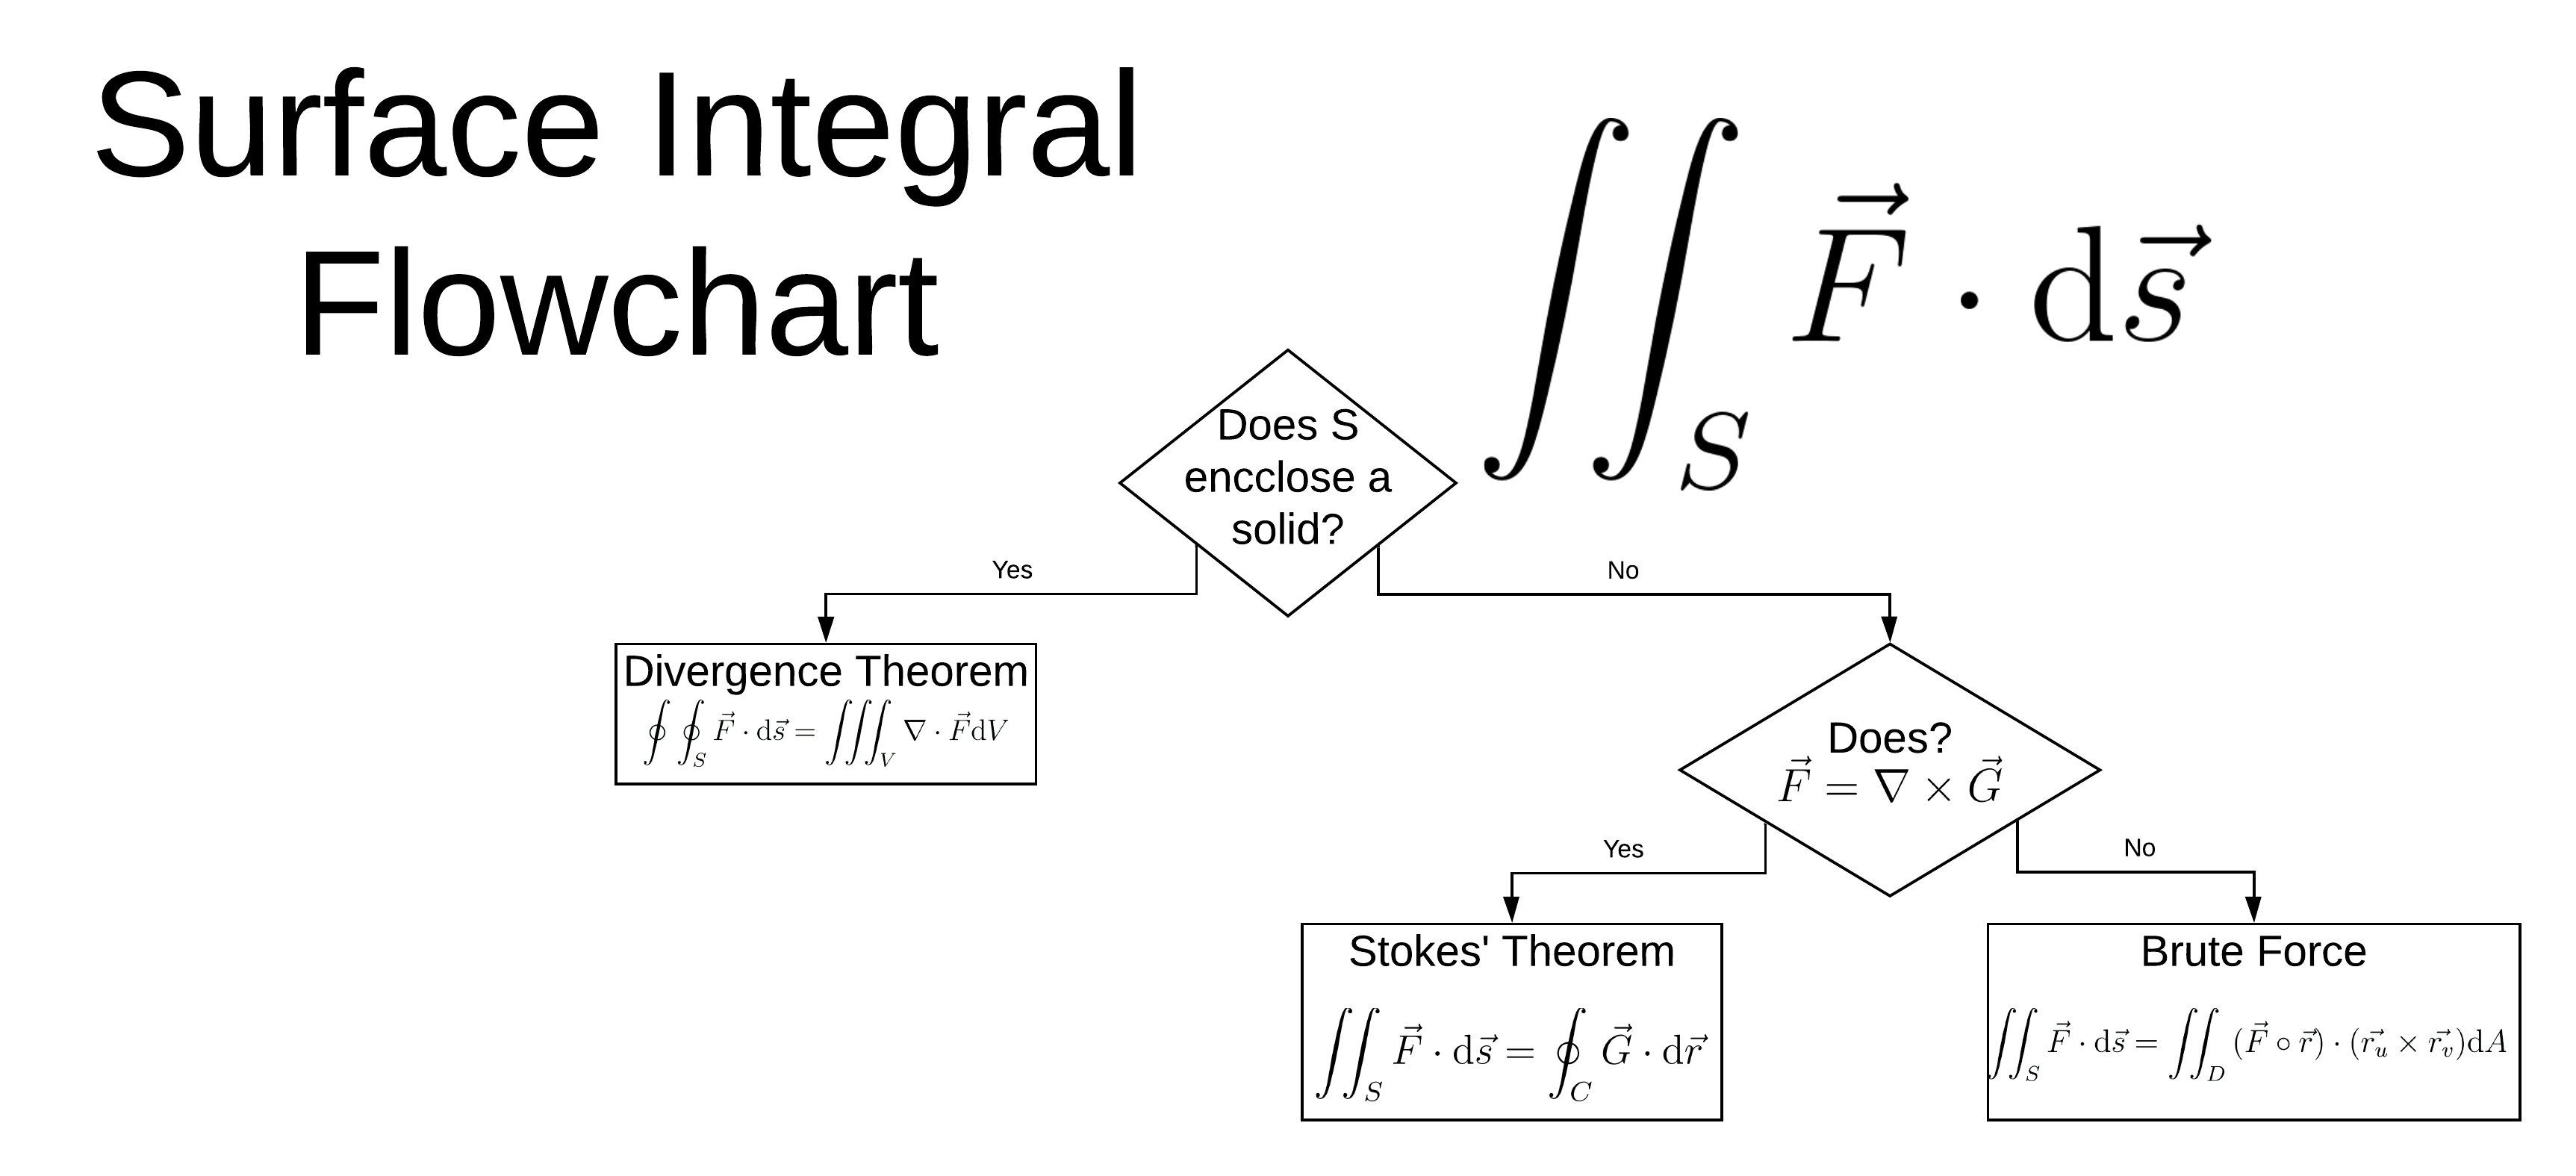
\includegraphics[width=\paperwidth]{Images/additionalMaterials/Surface_Integral_Flowchart}
\end{figure}

\pagebreak
\section{Worked Test Questions}
\noindent
These questions are modeled after actual exam questions a student might face in an undergraduate multivariable calculus course. The progression of the tests roughly follows the progression of topics covered.

\subsection{Test 1}
\begin{enumerate}
	\item Consider two intersecting lines $\vec{r_1}(t) = \langle 2, 3, 4t \rangle$ and $\vec{r_2}(t) = \langle 2+t, 3+2t, 0 \rangle$. Give the direction vector of each line. Find the equation of the plane which contains both lines. Draw a diagram of the lines, the plane, and the relevant vectors.\\
	\indent
	The direction vector of a line is the derivative of the position vector.
	\begin{itemize}
		\item Direction 1: $\langle 0, 0, 4 \rangle$
		\item Direction 2: $\langle 1, 2, 0 \rangle$
	\end{itemize}
	A the normal vector of the plane is the cross product of the direction vectors.
	\begin{itemize}
		\item $\vec{n} = \langle 0, 0, 4 \rangle \times \langle 1, 2, 0 \rangle = \langle -8, 4, 0 \rangle$
	\end{itemize}
	The lines intersect when $t = 0$ at $(2,3,0)$.
	So, the plane equation is: $\langle -8, 4, 0 \rangle \cdot \langle x-2, y-3, z \rangle = 0$
	
	\begin{figure}[h]
		\centering
		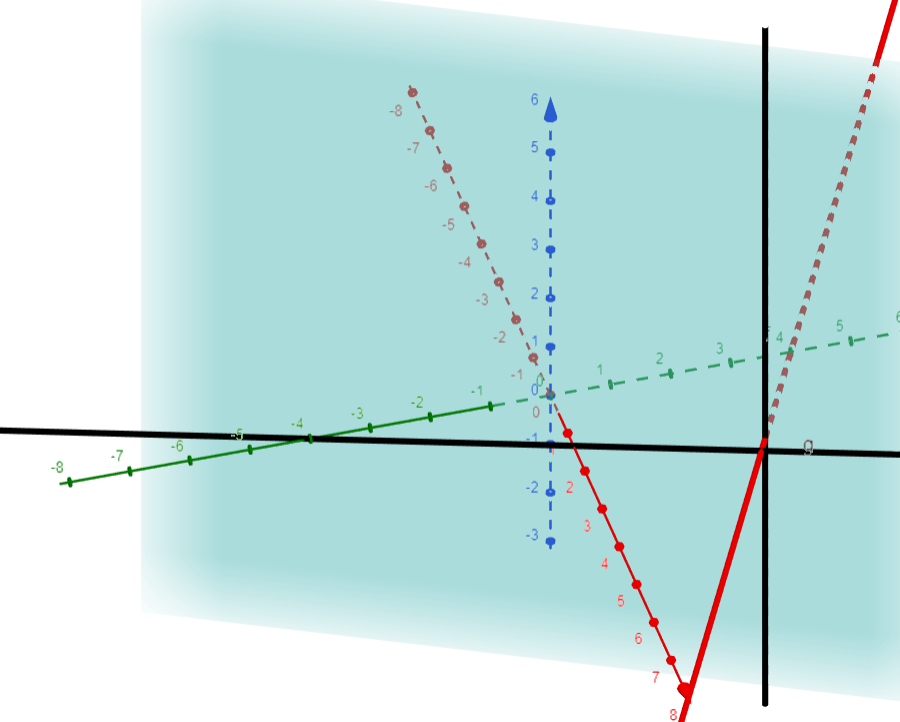
\includegraphics[scale=.5]{Images/additionalMaterials/test1_plane}
	\end{figure}
	
	\item Given the VVF $\vec{r}(t)\langle 10t, 7\cos{t}, 7\sin{t} \rangle$...
	\begin{enumerate}[label=\alph*.]
		\item Compute the unit tangent vector $\hat{T}(t)$ and the unit normal vector $\hat{N}(t)$.
		\begin{equation*}
			\hat{T} = \frac{\vec{r^\prime}(t)}{\norm{\vec{r^\prime}(t)}}	
		\end{equation*}
		\begin{equation*}
			\vec{r^\prime}(t) = \langle 10, -7\sin{t}, 7\cos{t} \rangle	
		\end{equation*}
		\begin{equation*}
			\norm{\vec{r^\prime}(t)} = \sqrt{10^2 + (-7\sin{t})^2 + (7\cos{t})^2} = \sqrt{149}	
		\end{equation*}
		\begin{equation*}
			\hat{T}(t) = \frac{1}{\sqrt{149}}\langle 10, -7\sin{t}, 7\cos{t} \rangle	
		\end{equation*}
		\begin{equation*}
			\hat{N}(t) = \frac{\mathrm{d}\hat{T}/\mathrm{d}t}{\norm{\mathrm{d}\hat{T}/\mathrm{d}t}}	
		\end{equation*}
		\begin{equation*}
			\frac{\mathrm{d}\hat{T}}{\mathrm{d}t} = \frac{1}{\sqrt{149}} \langle 0, -7\cos{t}, -7\sin{t} \rangle	
		\end{equation*}
		\begin{equation*}
			\norm{\frac{\mathrm{d}\hat{T}}{\mathrm{d}t}} = \frac{1}{\sqrt{149}}\sqrt{(-7\cos{t})^2 + (-7\sin{t})^2} = \frac{7}{\sqrt{149}}
		\end{equation*}
		\begin{equation*}
			\hat{N}(t) = \langle 0, -\cos{t},-\sin{t}\rangle
		\end{equation*}
		
		\item Show that $\hat{T}\perp\hat{N}$ for all $t$.\\
		If $\hat{T}\perp\hat{N}$, then $\hat{T}\cdot\hat{N} = 0$ for all $t$.\\
		\begin{align*}
			\hat{T} \cdot \hat{N} &= \frac{1}{\sqrt{149}}\langle 10, -7\sin{t}, 7\cos{t} \rangle \cdot \langle 0, -\cos{t}, -\sin{t}\rangle	\\
			&= \frac{1}{\sqrt{149}}(0 + 7\sin{t}\cos{t} - 7\sin{t}\cos{t}) = 0 \\
			&\implies \hat{T}\perp\hat{N}
		\end{align*}
	\end{enumerate}
	
	\item A cannon fires cannonballs with a speed of $20 \text{ m} / \text{s}$. Take acceleration due to gravity to be $g = 10 \text{m} / \text{s}^2$.
	\begin{enumerate}[label=\alph*.]
		\item Starting with a constant acceleration function $\vec{a} = \langle 0, -g \rangle$, find the velocity and position functions ($\vec{r^\prime}(t) \text{ and } \vec{r}(t)$ respectively) of the cannonball if the cannon is fired from an angle $\theta$ with respect to the horizontal. Assume the cannonball is initially positioned at the origin.\\
		We know that velocity is the integral of acceleration.
		\begin{equation*}
			\vec{v}(t) = \vec{r^\prime}(t) = \langle c_1, c_2-gt \rangle	
		\end{equation*}
		We are given that the initial speed is $20 \text{ m} / \text{s}$ at an angle $\theta$.
		\begin{equation*}
			\vec{v_0} = 20\langle \cos{\theta}, \sin{\theta} \rangle	
		\end{equation*}
		\begin{equation*}
			\vec{v}(t) = \langle 20\cos{\theta}, 20\sin{\theta}-gt \rangle	
		\end{equation*}
		We know that position is the integral of velocity.
		\begin{equation*}
			\vec{r}(t) = \langle 20t\cos{\theta} + c_1, 20t\sin{\theta} - \frac{1}{2}gt^2 + c_2 \rangle
		\end{equation*}
		We are given that the cannonball starts at the origin.
		\begin{equation*}
			\vec{r}(t) = \langle 20t\cos{\theta}, 20t\sin{\theta} - \frac{1}{2}gt^2 \rangle	
		\end{equation*}
		Taking $g = 10 \text{m} / \text{s}^2$,\\
		\begin{equation*}
			\vec{r}(t) = \langle 20t\cos{\theta}, 20t\sin{\theta}-5t^2 \rangle	
		\end{equation*}
			
		\item What angle $\theta$ should the cannon be fired to hit a target on the ground at a distance $40\text{ m}$ away?\\
		We want to find a point on the trajectory where $y = 0$ and $x = 40$.
		$y = 0$ when $t = 0, 4\sin{\theta}$. We can reasonably eliminate $t = 0$ because this is when the cannon first fires and $x = 0$.\\
		Plugging in $t = 4\sin{\theta}$ to the x-component of position when $x = 40$,
		\begin{align*}
			20\cos{\theta} \cdot 4\sin{\theta} &= 40 \\
			2\sin{\theta}\cos{\theta} &= 1 \\
			\sin{(2\theta)}=1, 2\theta &= \pi/2 \\
			\implies \theta &= \pi/4			
		\end{align*}
	\end{enumerate}
	
	\item Consider the following particle trajectory: $\vec{r}(t) = \langle R\cos{e^t}, R\sin{e^t}, \frac{h}{2\pi}e^t \rangle$ for $t \geq 0$. The shape of the trajectory is a helix with radius $R$ and vertical spacing $h$. Find the arc length function $s(t)$ of the trajectory starting with $s(0) = 0$. Give the arc length reparameterization of the helix.
	\begin{align*}
		s(t) &= \int_{0}^{t}{\norm{\vec{r^\prime}(\tau)}\mathrm{d}\tau}\\
		\vec{r^\prime}(t) &= \langle -Re^{t}\sin{e^t}, Re^{t}\cos{e^t}, \frac{h}{2\pi}e^{t} \rangle
	\end{align*}
	\begin{align*}
		\norm{\vec{r^\prime}(t)} &= \sqrt{(-Re^{t}\sin{e^t})^2 + (Re^{t}\cos{e^t})^2 + (\frac{h}{2\pi}e^t)^2} \\
		&= e^{t}\sqrt{R^2 + \frac{h^2}{4\pi^2}}
	\end{align*}
	\begin{equation*}
		s(t) = \int_{0}^{t}{e^{\tau}\sqrt{R^2 + \frac{h^2}{4\pi^2}}\mathrm{d}\tau} = \sqrt{R^2 + \frac{h^2}{4\pi^2}(e^{t} - 1)}
	\end{equation*}
	Solving for $t$,
	\begin{equation*}
		t = \ln{\left(\frac{s}{\sqrt{R^2 + \frac{h^2}{4\pi^2}}} + 1\right)}	
	\end{equation*}
	\begin{equation*}
		\vec{r}(s) = \left< R\cos{\left(\frac{s}{\sqrt{R^2 + \frac{h^2}{4\pi^2}}} + 1\right)}, R\sin{\left(\frac{s}{\sqrt{R^2 + \frac{h^2}{4\pi^2}}} + 1\right)}, \frac{h}{2\pi}\left(\frac{s}{\sqrt{R^2 +\frac{h^2}{4\pi^2}}} + 1\right) \right>
	\end{equation*}
	
	\item Let $\vec{r}(t)$ be the position function of a particle trapped on the surface of a sphere centered at the origin. Show that $\vec{r}(t)\perp\frac{\mathrm{d}}{\mathrm{d}t}\vec{r}(t)$ for all $t$.\\
	Since $\vec{r}(t)$ is on a sphere, $\norm{\vec{r}(t)} = R$ and $\vec{r}(t) \cdot \vec{r}(t) = R^2$.
	\begin{equation*}
		\frac{\mathrm{d}}{\mathrm{d}t}(\vec{r}(t) \cdot \vec{r}(t)) = 2\vec{r}(t) \cdot \vec{r^\prime}(t)	
	\end{equation*}
	\begin{equation*}
		\frac{\mathrm{d}}{\mathrm{d}t}(\vec{r}(t) \cdot \vec{r}(t)) = \frac{\mathrm{d}}{\mathrm{d}t}R^2 = 0
	\end{equation*}
	So, 
	\begin{equation*}
		2\vec{r}(t) \cdot \vec{r^\prime}(t) = 0
	\end{equation*}
	and 
	\begin{equation*}
		\vec{r}(t) \cdot \vec{r^\prime}(t) = 0	
	\end{equation*}
	\begin{equation*}
		\implies \vec{r}(t)\perp\vec{r^\prime}(t)	
	\end{equation*}
\end{enumerate}
\subsection{Test 2}
\begin{enumerate}
	\item Consider the function $f(x,y) = x^2 - 2x + y^2 - 4y + 7$.\\
	\begin{enumerate}[label=\alph*.]
		\item Find equations for an plot (if possible) the C-level curves of $f$ for $C = 3$ and $C = 1$.\\
		\indent
		We will try to find the level curve for any $C$ and then plug in 1 and 3.\\
		$x^2 - 2x + y^2 - 4y + 7 = C$\\
		$x^2 - 2x + 1 + y^2 - 4y + 4 = C-2$\\
		$(x-1)^2 + (y-2)^2 = C-2$: A circle of radius $\sqrt{C-2}$ centered at $(1,2)$.\\
		For $C = 1$, the level curve does not exist because the circle would have a radius of $\sqrt{2-1} = \sqrt{-1}$.\\
		For $C = 3$, the level curve is $(x-1)^2 + (y-2)^2 = 1$.
		
		\begin{figure}[h]
			\centering
			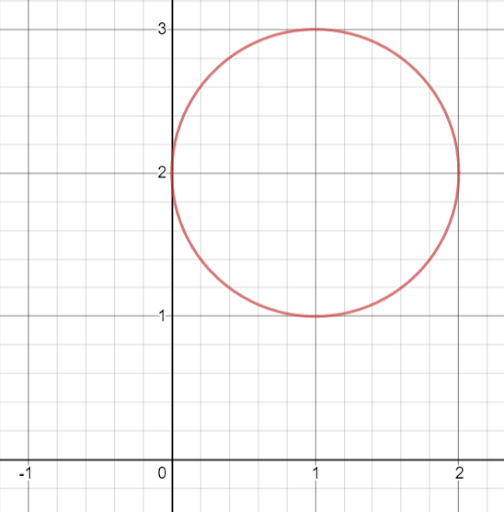
\includegraphics[scale=.24]{Images/additionalMaterials/test2_circle}
		\end{figure}
		
		\item Compute $\nabla f$.\\
		\indent
		$\nabla f = \langle f_x, f_y\rangle = \langle 2x-2, 2y-4 \rangle$\\
		
		\item Find the equation of the plane tangent to the surface $z = f(x,y)$ at the point $(x_0, y_0, z_0) = (2,4,7)$.\\
		\indent
		$\vec{n} = \langle f_x, f_y, -1\rangle = \langle 2x-2, 2y-4, -1 \rangle$\\
		At $(2,4,7)$, $\vec{n} = \langle 2, 7, -1 \rangle$.\\
		So, the plane equation is $\langle 2, 7, -1 \rangle \cdot \langle x-2, y-4, z-7 \rangle = 0$.\\
		
		\item Perform one iteration of gradient descent on $f(x,y)$ with a learning rate $delta = 1/4$ starting from the point $(x_0,y_0) = (2,4)$.\\
		\indent
		$(x_n, y_n) = (x_{n-1},y_{n-1}) - \delta\nabla f$\\
		$(x_0, y_0) = (2,4)$, $\delta = 1/4$, and $\nabla f = \langle 2x-2, 2y-4 \rangle$\\
		$(x_1, y_1) = (2,4) - \frac{1}{4} \langle 2(2)-2, 2(4)-4 \rangle$\\
		$= (3/2, 3)$\\
	\end{enumerate}

	\item Recall that for a differentiable function $f(x,y)$ and the unit vector $\hat{u} = \langle a, b \rangle$, we proved that $D_{\hat{u}}f = \nabla f \cdot \hat{u}$.
	\begin{enumerate}[label=\alph*.]
		\item Prove the statement "The gradient is the direction of steepest ascent" by showing that the directional derivative $D_{\hat{u}}f$ is maximized when $\hat{u}\parallel\nabla f$.\\
		\indent
		$D_{\hat{u}}f = \nabla f \cdot \hat{u}=\norm{\nabla f}\norm{\hat{u}}\cos{\theta} = \norm{\nabla f}\cos{\theta}$\\
		This value is maximized when $\theta$ is a multiple of $2\pi$, meaning that the angle between $\nabla f$ and $\hat{u}$ is 0. This means that the maximum value of the directional derivative, the direction of steepest ascent, is in the same direction as $\nabla f$.\\
			
		\item State the limit definition of the directional derivative $D_{\hat{u}}f$. Starting from that definition, prove that $D_{\hat{u}}f = \nabla f\cdot\hat{u}$.\\
		$D_{\hat{u}}f = \lim_{h \to 0}{\frac{f(x+ah, y+bh)}{h}}$ and $\hat{u}=\langle a, b \rangle$.\\
		$= \lim_{h \to 0}{\frac{f(x+ah, y+bh) - f(x+ah, y)}{h} + \frac{f(x+ah, y) - f(x,y)}{h}}$\\
		$= b\lim_{h \to 0}{\frac{f(x, y+bh) - f(x,y)}{bh}} + a\lim_{h \to 0}{\frac{f(x+ah, y) - f(x,y)}{ah}}$\\
		$= bf_y + af_x = \langle f_x, f_y \rangle \cdot \langle a, b \rangle = \nabla f \cdot \hat{u}$\\
	\end{enumerate}
	
	\item Use the method of Lagrange Multipliers to find the maximum of the product of two numbers $x$ and $y$ given that $(x,y)$ is a coordinate pair in the 1st quadrant located on the unit circle centered at the origin. Begin by stating the objective function $f(x,y)$ and the constraint equation $g(x,y) = k$.\\
	\indent
	Objective Function: $f(x,y) = xy$\\
	Constraint Equation: $g(x,y) = x^2 + y^2 = 1$, $x \geq 0$ and $y \geq 0$.\\
	$F(x,y,\lambda) = xy + \lambda(1-x^2-y^2)$\\
	$\frac{\partial F}{\partial x} = y-2\lambda x$, $\frac{\partial F}{\partial y} = x-2\lambda y$, and $\frac{\partial F}{\partial\lambda} = 1-x^2-y^2$.\\
	$\langle y-2\lambda x, x-2 \lambda y, 1-x^2-y^2 \rangle = \vec{0}$\\
	$\begin{cases}
		y = 2\lambda x \\
		x = 2\lambda y \\
		x^2 + y^2 = 1
	\end{cases} 
	\implies
	\begin{cases}
		\lambda = 1/2 \\
		x = 1/\sqrt{2} \\
		y = 1/\sqrt{2}
	\end{cases}$\\
	So, the maximum product is $\frac{1}{\sqrt{2}} \cdot \frac{1}{\sqrt{2}} = \frac{1}{2}$ at $\left(\frac{1}{\sqrt{2}}, \frac{1}{\sqrt{2}}\right)$\\
	
	\item The function $p(x,y) = \frac{1}{\pi}\exp{\left(-(x-a)^2 - (y-b)^2\right)}$ is the probability density function of a bivariate normal distribution with mean $(a,b)$ and standard deviation $\frac{1}{\sqrt{2}}$. Show that the global maximum of $p(x,y)$ occurs at $(a,b)$.\\
	\indent
	$p_x = \frac{1}{\pi}(-2(x-a))\exp{(-((x-a)^2 + (y-b)^2))}$\\
	$p_y = \frac{1}{\pi}(-2(y-b))\exp{(-((x-a)^2 + (y-b)^2))}$\\
	$p_x = 0$ when $x=a$ and $p_y = 0$ when $y=b$\\
	$\implies (a,b)$ is a critical point.\\
	$p_{xx} = \frac{1}{\pi}(-2(y-b))\exp{(-((x-a)^2 + (y-b)^2))} - 2\exp{(-((x-a)^2 + (y-b)^2))}$\\
	$= \frac{1}{\pi}(4(x-a)^2 - 2)\exp{(-((x-a)^2 + (y-b)^2))}$\\
	Similarly, $p_{yy} = \frac{1}{\pi}(4(y-b)^2 - 2)\exp{(-((x-a)^2 + (y-b)^2))}$\\
	$p_{xy} = p_{yx} = \frac{4}{\pi}(x-a)(y-b)\exp{(-((x-a)^2 + (y-b)^2))}$\\
	$p_{xx}(a,b) = \frac{-2}{\pi}$, $p_{yy}(a,b) = \frac{-2}{\pi}$, and $p_{xy}(a,b) = p_{yx}(a,b) = 0$\\
	$H(a,b) = \begin{bmatrix}
		\frac{-2}{\pi} & 0 \\
		0 & \frac{-2}{\pi}
	\end{bmatrix}$\\
	$\det{(H(a,b))} = \frac{4}{\pi^2}$\\
	$(a,b)$ is an extrema because $\det{(H(a,b))} > 0$.\\
	Since $f_{xx}(a,b) < 0$ and $f_{yy}(a,b) < 0$, $(a,b)$ is a maximum.\\
	$(a,b)$ is a global maximum because $p(x,y)$ is strictly decreasing as you move away from $(a,b)$.\\
	
	\item Let the C-level curve of the function $f(x,y)$ be parameterized by the VVF $\vec{r}(t) = \langle x(t), y(t) \rangle$. Use the chain rule to show that $\nabla f(\vec{r}(t))\perp\vec{r^\prime}(t)$ for all $t$.\\
	\indent
	Since $\vec{r}(t)$ parameterizes a C-level curve of $f$, $f\circ\vec{r}(t) = C$. Where $C$ is a constant.\\
	$\frac{\mathrm{d}}{\mathrm{d}t}(f\circ\vec{r}(t)) = \frac{\mathrm{d}}{\mathrm{d}t}C$\\
	$\frac{\partial f}{\partial x}\frac{\mathrm{d}x}{\mathrm{d}t} + \frac{\partial f}{\partial y}\frac{\mathrm{d}y}{\mathrm{d}t} = 0$\\
	$\left<\frac{\partial f}{\partial x}, \frac{\partial f}{\partial y}\right> \cdot \left<\frac{\mathrm{d}x}{\mathrm{d}t}, \frac{\mathrm{d}y}{\mathrm{d}t}\right> = 0$\\
	$\nabla f(\vec{r}(t)) \cdot \vec{r^\prime}(t) = 0$\\
	$\implies \nabla f(\vec{r}(t))\perp\vec{r^\prime}(t)$\\
\end{enumerate}
\subsection{Test 3}

\begin{enumerate}[label=\arabic*.]
	\item
		Write the integral definition of the Laplace transform.
	\item 
		Find the Laplace transform of the following functions. Be sure to give the domains. Use the integral definition for (a) and (e). Be sure to state the domain of the transformed function and any rules of Laplace transforms you use.
		\begin{enumerate}[label = (\alph*)]
			\item
				\begin{equation*}
					f(x) = e^x
				\end{equation*}
			\item
				\begin{equation*}
					h(t) = \sin{t} + 2\cos{3t}
				\end{equation*}
			\item
				\begin{equation*}
					j(t) = e^{3t}\left(t^2 + 3t + 2\right)
				\end{equation*}
			\item
				\begin{equation*}
					b(t) = \dd{}{t}{(e^{3t+1} + e^{1-t})}
				\end{equation*}
%			\item
%				\begin{equation*}
%					\delta(x) = \lim\limits_{a \to 0}{\frac{1}{\abs{x}\sqrt{\pi}}e^{(x/a)^2}}
%				\end{equation*}
		\end{enumerate}
	\item
		Find the inverse Laplace transform of the following functions.
		\begin{enumerate}[label=(\alph*)]
			\item
				\begin{equation*}
					F(s) = \frac{1}{1+s}
				\end{equation*}
			\item
				\begin{equation*}
					H(s) = \frac{s^2+2s+1}{s^3 - 4s^2 + 5s - 2}					
				\end{equation*}
			\item
				\begin{equation*}
					J(s) = \frac{s-4}{s^2 -8s + 32}
				\end{equation*}
			\item
				\begin{equation*}
					A(s) = \frac{768}{(2s+3)^5}
				\end{equation*}
		\end{enumerate}
	\item
		Find the general solution to the following differential equation using one of the methods you learned previously and by Laplace transform. Show that the two methods give the same answer.
		\begin{equation*}
			2y'' - 3y' + y = 10\sin{x}
		\end{equation*}
	\item
		Solve the following IVP by Laplace transform.
		\begin{equation*}
			\begin{cases}
				2y'' + 4y' - 6y = te^{-3t} \\
				y'(0) = 0 \\
				y(0) = 1
			\end{cases}
		\end{equation*}
\end{enumerate}
\subsection{Test 4}
\begin{enumerate}
	\item For each of the following, determine if $\vec{F}$ is conservative. Then evaluate $\int\limits_{C}{\vec{F}\cdot\mathrm{d}\vec{r}}$.
	\begin{enumerate}[a.]
		\item $\vec{F}=\langle xz, x^2z, xy^2z\rangle$ and $C$ given by $\vec{r}(t)=\langle t,e^{-t},e^t\rangle, 0\leq t\leq 1$.\\
		$\nabla\times\vec{F}=\langle 2xyz-x^2,x-y^2z,2xz\rangle$\\
		Since $\nabla\times\vec{F}\neq\vec{0}$, $\vec{F}$ isn't conservative.\\
		$\vec{F}\circ\vec{r}=\langle te^t, t^2e^t,te^{-2t}e^t\rangle$\\
		$=\vec{r^\prime}(t)=\langle 1,-e^{-t},e^t\rangle$\\
		$\left(\vec{F}\circ\vec{r}\right)\cdot\vec{r^\prime}(t)=te^t-t^2+t$\\
		$\int\limits_{C}{\vec{F}\cdot\mathrm{d}\vec{r}}=\int_{0}^{1}{\left(te^t-t^2+t\right)\mathrm{d}t}$\\
		$=\frac{1}{2}-\frac{1}{3}+\lvert te^t\rvert_{0}^{1}-\int_{0}^{1}{e^t\mathrm{d}t}$\\
		$=1+\frac{1}{2}-\frac{1}{3}=\frac{7}{6}$\\
		
		\item $\vec{F}=\left<\sqrt{\frac{yz}{x}},\sqrt{\frac{xz}{y}},\sqrt{\frac{xy}{z}}\right>$ and $C$ given by $\vec{r}=\langle\cos{t},\sin{t},\sin{(4t)}\rangle, 0\leq t\leq 2\pi$.\\
		\indent
		$\vec{F}=\nabla(2\sqrt{xyz})$
		$\implies\vec{F}$ is conservative.
		$\vec{r}(0)=\vec{r}(2\pi)$\\
		$\implies C$ is a circulation.
		Since $\vec{F}$ is conservative and $C$ is a circulation, $\oint\limits_{C}{\vec{F}\cdot\mathrm{d}\vec{r}}=0$\\
		
		\item $\vec{F}=\langle yz, xz, xy\rangle$ and $C$ given by $\vec{r}(t)=\langle 2t^2, e^{1-t^2}, \tan^{-1}{(t^2/2)}\rangle, 0\leq t\leq\sqrt{2}$.\\
		$\vec{F}=\nabla(xyz)$\\
		$\implies\vec{F}$ is conservative.\\
		$\int\limits_{C}{\vec{F}\cdot\mathrm{d}\vec{r}}=\int\limits_{C}{\nabla f\cdot\mathrm{d}\vec{r}}=f(\vec{r}(\sqrt{2}))-f(\vec{r}(0))$\\
		$=\frac{4\pi}{4e}-0=\frac{\pi}{e}$\\
	\end{enumerate}
	
	\item Let the surface $S$ be the portion of the paraboloid $z=8-\frac{x^2}{2}-\frac{y^2}{2}$ that lies above the xy-plane. Let $\vec{F}(x,y,z)=\left< \frac{x}{\sqrt{x^2+y^2}}, \frac{y}{\sqrt{x^2+y^2}}, 0\right>$.
	\begin{enumerate}[a.]
		\item Parameterize $S=\vec{r}(u,v)$ with appropriate bounds for $u$ and $v$.\\
		\indent
		The paraboloid is above the xy-plane when $z\geq0$.\\
		$8-\frac{x^2}{2}-\frac{y^2}{2}=\geq 0$\\
		$x^2+y^2\leq 16$\\
		This a circle with radius 4. So, we'll describe the region in polar form.\\
		$S=\left\{(r,\theta)|0\leq r\leq 4, 0\leq\theta\leq 2\pi\right\}$\\
		$\vec{r}(u,v)=\langle u\cos{v},u\sin{v},8-\frac{1}{2}u^2\rangle$, $0\leq u\leq 4$ and $0\leq v\leq 2\pi$.\\
		
		\item Compute the surface area of $S$.\\
		\indent
		$A-\iint\limits_{D}{\norm{\vec{r_u}\times\vec{r_v}}\mathrm{d}A}$\\
		$\vec{r_u}=\langle\cos{v},\sin{u},-u\rangle$\\
		$vec{r_v}=\langle -u\sin{v},u\cos{v},0\rangle$\\
		$\vec{r_u}\times\vec{r_v}=\langle u^2\cos{v},u^2\sin{v},u\rangle$\\
		$\norm{\vec{r_u}\times\vec{r_v}}=u\sqrt{1+u^2}$\\
		$A=\int_{0}^{2\pi}{int_{0}^{4}{u\sqrt{1+u^2}\mathrm{d}u}\mathrm{d}v}$\\
		$=2\pi\int_{0}^{4}{u\sqrt{1+u^2}\mathrm{d}u}$\\
		$=\pi\int_{1}^{17}{\sqrt{w}\mathrm{d}w}$\\
		$=\pi\frac{34\sqrt{17}-2}{3}$\\
		
		\item Compute the flux, $\Phi$, of $\vec{F}$ through $S$.\\
		\indent
		We will assume that the surface is outward-oriented, so that $\Phi$ is positive.\\
		$\Phi=\iint\limits_{D}{\left(\vec{F}\circ\vec{r}\right)\cdot\left(\vec{r_u}\times\vec{r_v}\right)\mathrm{d}A}$\\
		$\vec{F}\circ\vec{r}=\langle\cos{v}\sin{v},0\rangle$\\
		$\left(\vec{F}\circ\vec{r}\right)\cdot\left(\vec{r_u}\times\vec{r_v}\right)=u^2$\\
		$\Phi=\int_{0}^{2\pi}{\int_{0}^{4}{u^2\mathrm{d}u}\mathrm{d}v}$\\
		$=\frac{128\pi}{3}$\\
	\end{enumerate}
	
	\item Consider a 3D vector field $\vec{F}(x,y,z)=\langle P(x,y,z),Q(x,y,z),R(x,y,z)\rangle$ and a scalar function of two variables $f(x,y)$. Determine which of the following expressions is defined. If it is defined, evaluate it. If it is not defined, explain why. If you can deduce the value of the expression from a theorem, do so and state the theorem.
	\begin{enumerate}[a.]
		\item $$\nabla f\cdot\vec{F}$$
		\indent
		This operation is not defined because $\nabla f$ is a 2D vector, and the output of $\vec{F}$ is a 3D vector.\\
		
		\item $$\nabla\times\nabla f$$
		\indent
		If we allow the cross product in 2D to return a scalar that is the signed area spanned by the two vectors, then\\
		$\nabla\times\nabla f=f_{yx}-f_{xy}=0$\\
		
		\item $$\nabla\times(\nabla\cdot\vec{F})$$
		\indent
		This operation is not defined because $\nabla\cdot\vec{F}$ results in a scalar function, and the curl of a scalar function is not defined.\\
		
		\item $$\nabla\cdot(\nabla\times\vec{F})$$
		\indent
		This operation is defined and always has a value of 0 if $\vec{F}$ is twice differentiable. The proof of which is below.\\
		Let $\vec{F}(x,y,z)=\langle P(x,y,z),Q(x,y,z),R(x,y,z),\rangle$\\
		$\nabla\cdot(\nabla\times\vec{F})=\nabla\cdot\langle R_y-Q_z,P_z-R_x,Q_x-P_y\rangle$\\
		$=R_{yx}-Q_{zx}+P_{zy}-R_{xy}+Q_{xz}-P_{yz}=0$ by Fubini's Theorem\\
	\end{enumerate}

	\item Consider the vector field $\vec{F}(x,y,z)=\langle -z,2y,x\rangle$. Find the integral curve of $\vec{F}$ with initial conditions $\vec{r}(0)=\langle 5,1,0\rangle$.\\
	\indent
	We need to solve a system of differential equations.\\
	$\begin{cases}
		x^\prime = -z \\
		y^\prime = 2y \\
		z^\prime = x
	\end{cases}$\\
	$y(t)=Ce^{2t}$ and applying initial conditions, $y(t)=e^{2t}$\\
	$\begin{cases}
		x^\prime = -z \\
		z^\prime = x
	\end{cases}$\\
	$z(t)=A\cos{t}+B\sin{t}$ and $x(t)=B\cos{t}-A\sin{t}$\\
	Applying initial conditions, $z(t)=5\sin{t}$ and $x(t)=5\cos{t}$\\
	So, $\vec{r}(t)=\langle 5\cos{t},e^{2t}, 5\sin{t}\rangle$\\
	
	\item State and prove the Fundamental Theorem of Calculus for Line Integrals.\\
	\indent
	\begin{theorem}[FTC for Line Integrals]
		Let $\vec{r}(t)$ parameterize $C$ on $a\leq t\leq b$.\\
		$\int\limits_{C}{\nabla f\cdot\mathrm{d}\vec{r}}=f(\vec{r}(b))-f(\vec{r}(a))$
	\end{theorem}
	\begin{proof}
		$\int\limits_{C}{\nabla f\cdot\mathrm{d}\vec{r}}=\int_{a}^{b}{(\nabla f\circ\vec{r})\cdot\vec{r^\prime}\mathrm{d}t}$\\
		$=\int_{a}^{b}{\frac{\mathrm{d}}{\mathrm{d}t}(f\circ\vec{r})\mathrm{d}t}$\\
		$f(\vec{r}(b))-f(\vec{r}(a))$
	\end{proof}
\end{enumerate}
\section{Online Resources}
\noindent
Below is a list of other useful resources for learning differential equations. Most are freely accessible online.
\begin{itemize}
	\item
		\href{http://tutorial.math.lamar.edu/Classes/DE/DE.aspx}{Paul's Online Notes} -- Goes deeper than this text and has additional practices problems.
	\item
		\href{https://www.khanacademy.org/math/differential-equations}{Khan Academy} -- Video lectures and practice problems.
	\item
		\href{https://www.youtube.com/playlist?list=PLD4B0062CA82D73FB}{PatrickJMT} -- YouTube series focused mostly on solving example problems.
	\item
		\href{https://ocw.mit.edu/courses/mathematics/18-03sc-differential-equations-fall-2011/}{MIT OCW 18.03SC} -- Complete series of lectures, recitations, assignments, practice problems, lecture notes, and exams needed for independent study.
	\item
		\href{https://www.math.ust.hk/~machas/differential-equations.pdf}{Jeffery R. Chasnov: Differential Equations} -- Online textbook from the Hong Kong University of Science and Technology. Adapted from Coursera's Differential Equations for Engineers.
\end{itemize}
\section{Contributors}
Special thanks to everyone who made contributions to this project on \href{https://github.com/wmboyles/Math-Summaries}{Github}.
They are listed in order of number of commits as \texttt{name (GitHub username)}.

\begin{center}
    \begin{tabular}{ c c c }
    	William Boyles (\href{https://github.com/wmboyles}{wmboyles}) & Nate (\href{https://github.com/aneziac}{aneziac}) & Ashwin M  (\href{https://github.com/Suzukazole}{Suzukazole}) \\
		आदित्य देव (\href{https://github.com/dev-aditya}{dev-aditya}) & Calvin McPhail-Snyder (\href{https://github.com/esselltwo}{esselltwo}) & Robert Washbourne (\href{https://github.com/rawsh}{rawsh}) \\
	\end{tabular}
\end{center}


\backmatter
\end{document}